\label{ch:qg}
\chapter{Prospects}
For the resolved analysis, signal jets are quark enriched and background jets are gluon dominated. By classifying jets in the event as quark or gluon initiated, less background would contaminate the signal region. Figure~\ref{fig:diag_pdgid} shows the PDGID for the truth parton matched to the jet (meaning the highest energy parton in the jet catchment area) in events passing the resolved signal region selections. PDGID = -1 corresponds to pileup jets, 0 < PDGID < 6 correspond to quarks and PDGID = 21 corresponds to gluons. From this Figure, it is evident that a notable fraction of the background (all background events that passed the resolved SR are used) that contaminates the signal region contains gluon jets, especially for the sub-leading jet. 

As gluons jets have more constituents and therefore more tracks ($n_{trk}$), background jets generally have more tracks than the signal jets. This is shown in Figure~\ref{fig:diag_ntrk}. Therefore, by cutting on the number of tracks in a jet, quark and gluon jets may be distinguished (i.e. jets with less than a given number of tracks are classified as a quark, otherwise the jet is classified as a gluon.) Moreover, as the momentum of the jet increases the number of tracks also increases logarithmically [Cite nachman thesis Natasha], and improves tagging efficiency by about 10\% relative to a constant cut on the number of tracks. Therefore by applying a cut on the number of tracks that scales with the $ln(p_{T})$ is more powerful than a threshold cut on the number of tracks. Figures \ref{fig:bkg_heatmap}-\ref{fig:sig700_heatmap} show normalized heat maps of $ln(p_{T})$ vs the number of reconstructed tracks for the background and HVT $Z'$ signals. This information is also shown in table \ref{qgtable}. In these plots it is evident that the number of tracks in the background jets grows more quickly with $ln(p_{T})$ than for the signal jets. This is expected given that the signal is quark dominated and the background is gluon dominated. 

In Figure~\ref{fig:quark_gluon_roc} is the ROC Curve for quark gluon tagging with cut on the number of tracks in a jet that depends on $ln(p_{T})$. The sum of the backgrounds in the signal region were used for this curve. Here the quark tagging efficiency is the ratio of quarks tagged as quarks to the total number of quarks in the signal region. The gluon rejection is calculated as the reciprocal of the gluon tagging efficiency. For example, choosing a 90\% efficient working point with a rejection of 1.4 corresponds to a slope of 4 and intercept of -5. Tagging both jets in this analysis would yield an efficiency of $90\%^{njets}$. Focusing on the background in Figure~\ref{fig:qg_s_root_b}, this cut helps minimize gluon contamination in the signal region. Also, from these heat maps it is obvious that the number of tracks in gluon jets grows more quickly than those in quark jets.
\pagebreak

\begin{figure}[h!]
  \centering
  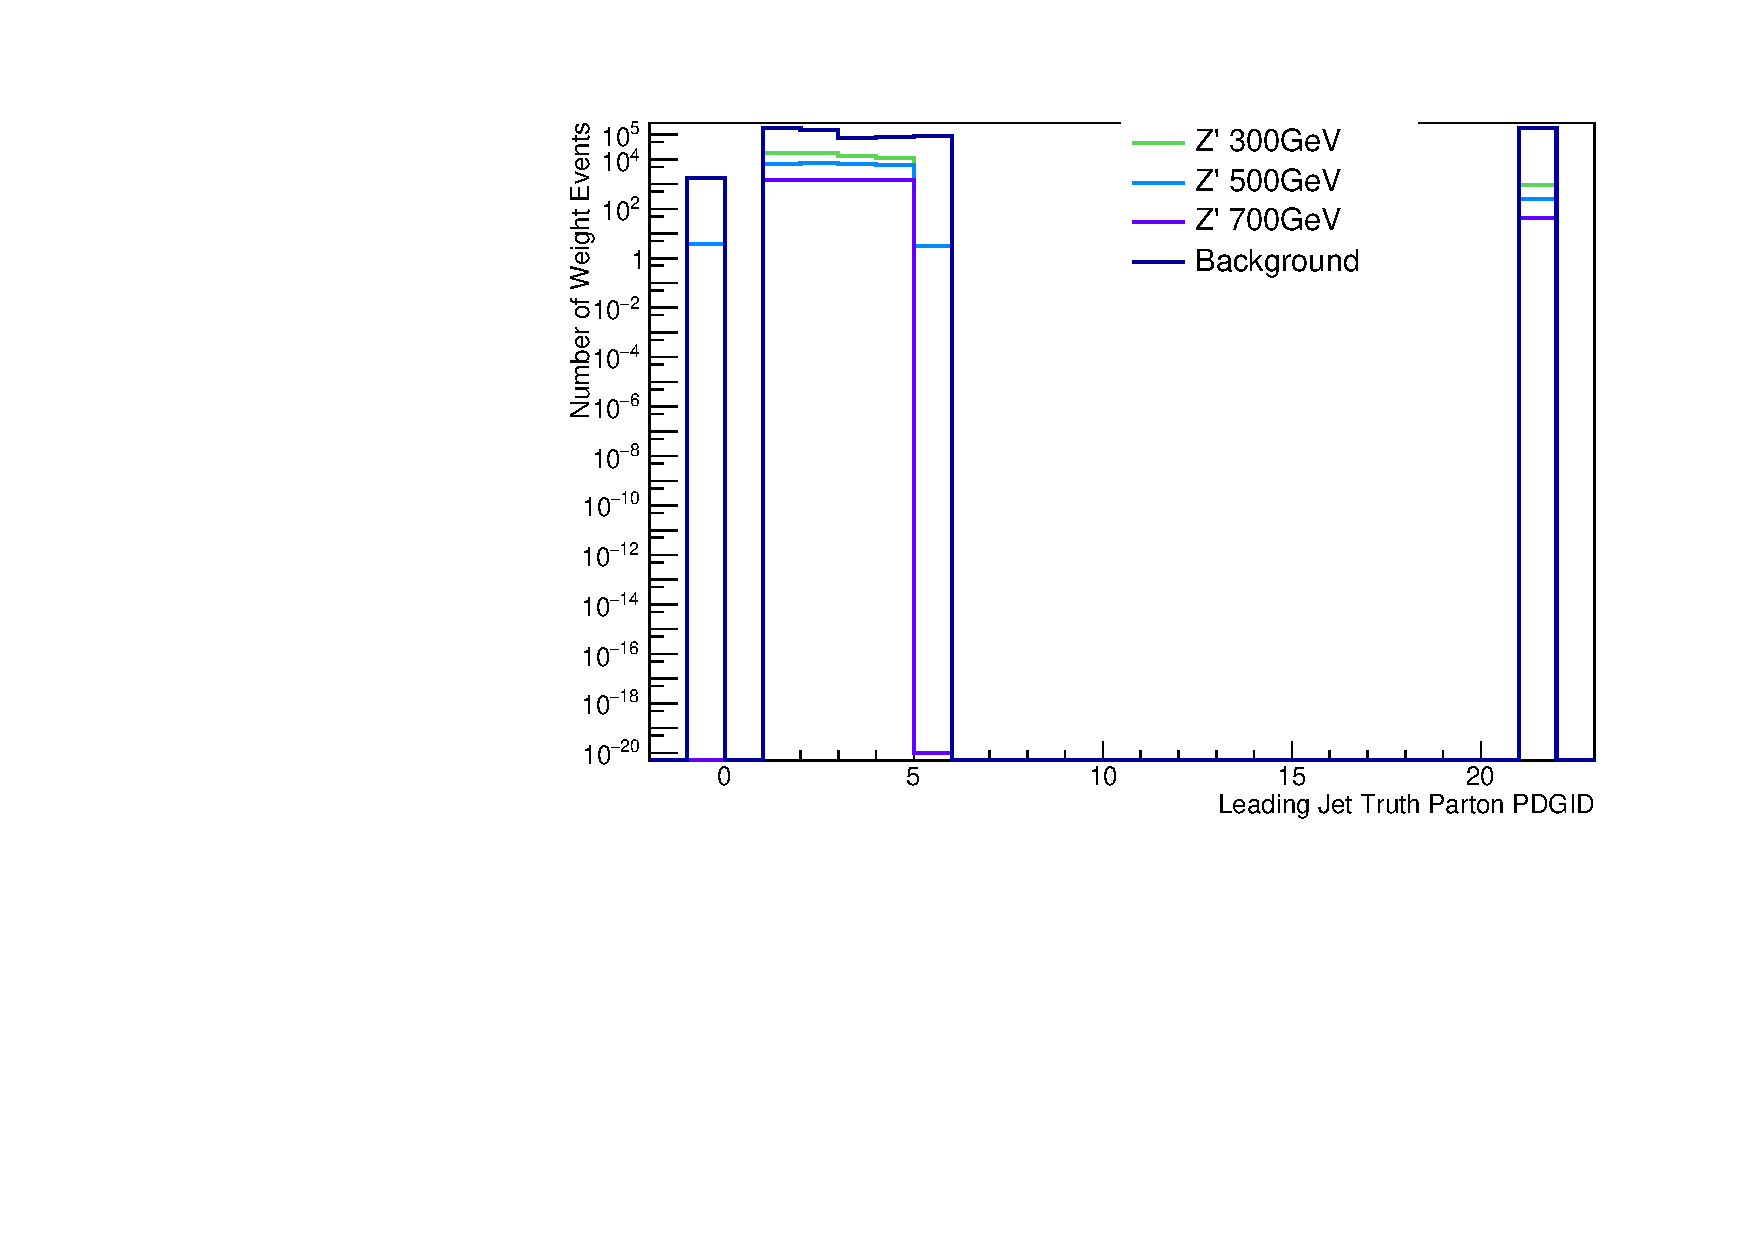
\includegraphics[width=0.45\hsize]{figures/QGT/sigWJ1_pdgid_Pass_Res_GGF_WW_SR.pdf}
 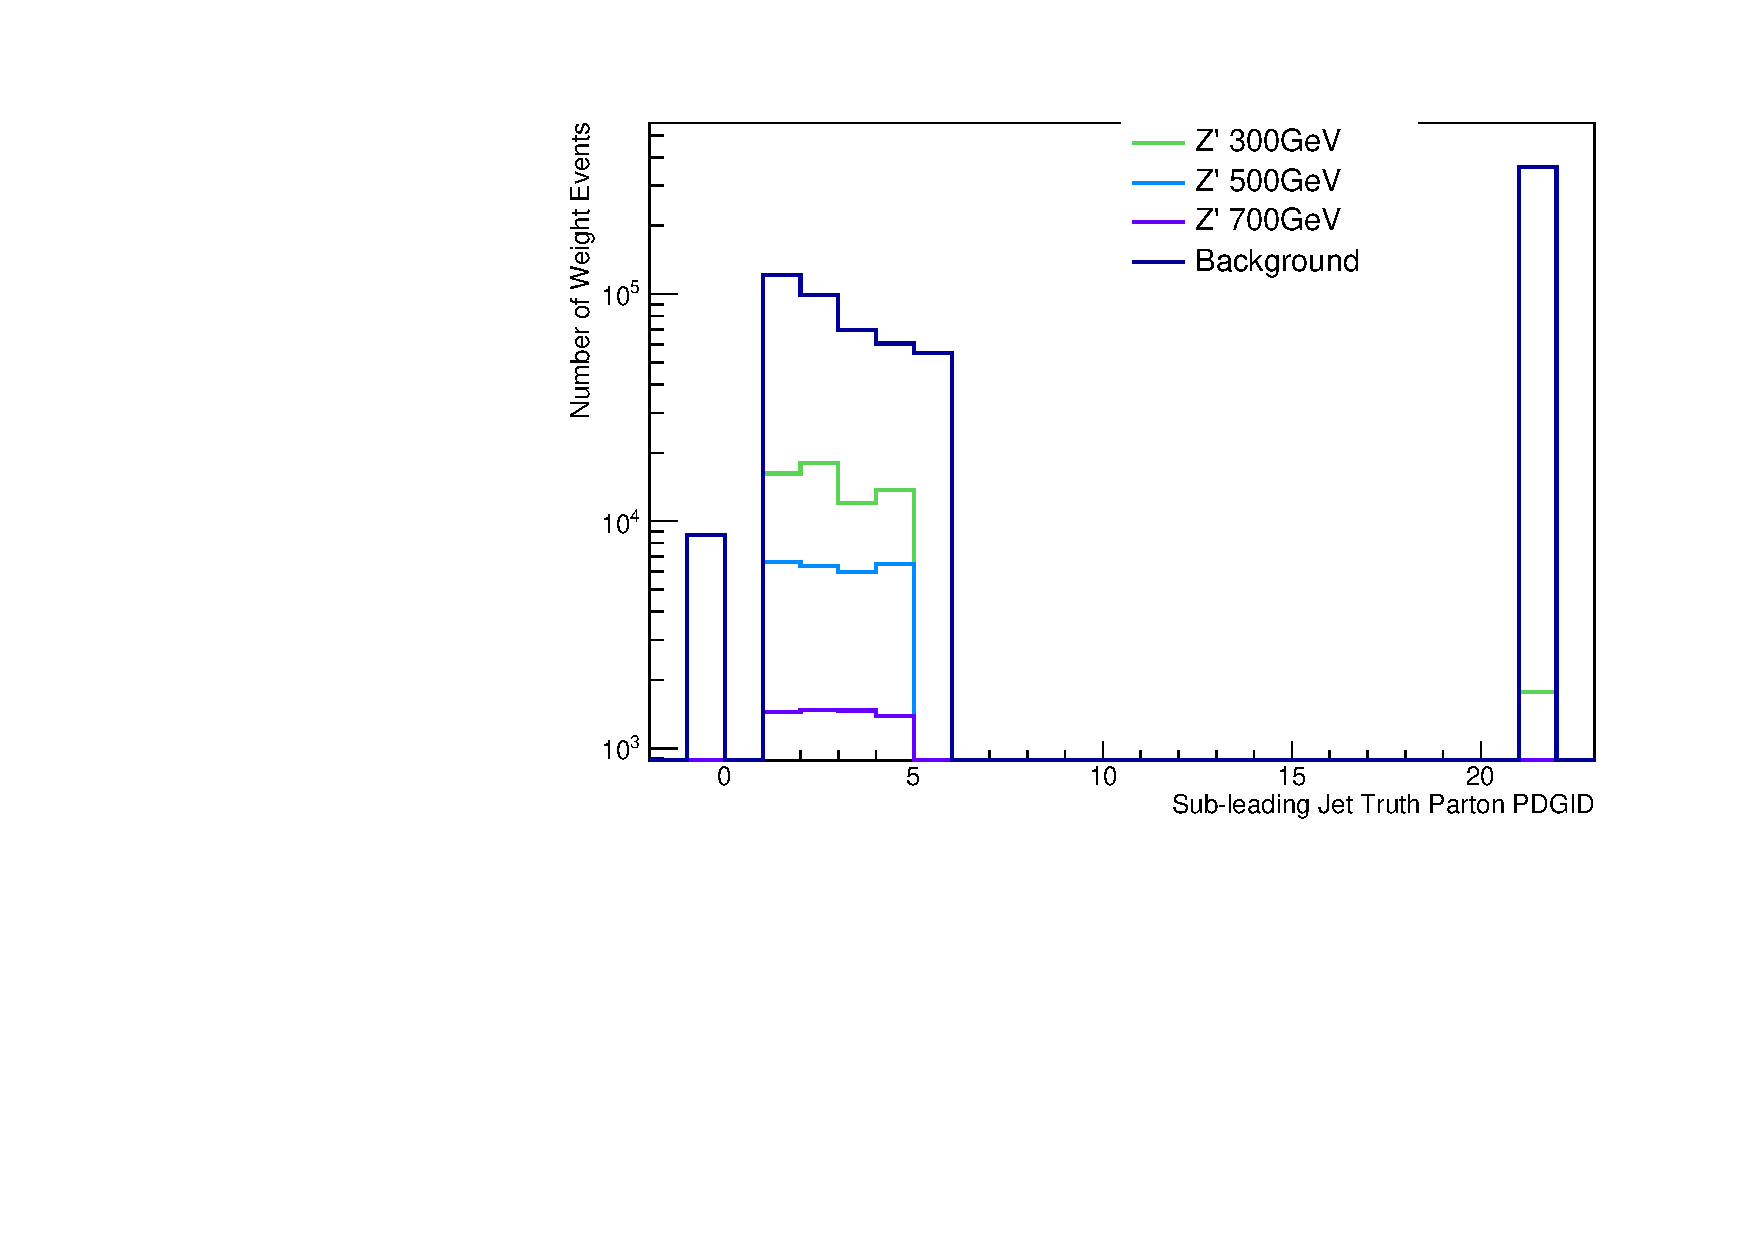
\includegraphics[width=0.45\hsize]{figures/QGT/sigWJ2_pdgid_Pass_Res_GGF_WW_SR.pdf}
  \caption{PDGID of the truth-level parton matched to the small-R jets passing the Resolved GGF WW Signal Region selections for the (a) Leading (b) Sub-Leading jets . These distributions are shown for 300, 500, and 700GeV Z' signals and the background (all simulated backgrounds that pass SR selections).}
  \label{fig:diag_pdgid}
\end{figure}
\FloatBarrier



\begin{figure}[h!]
  \centering
  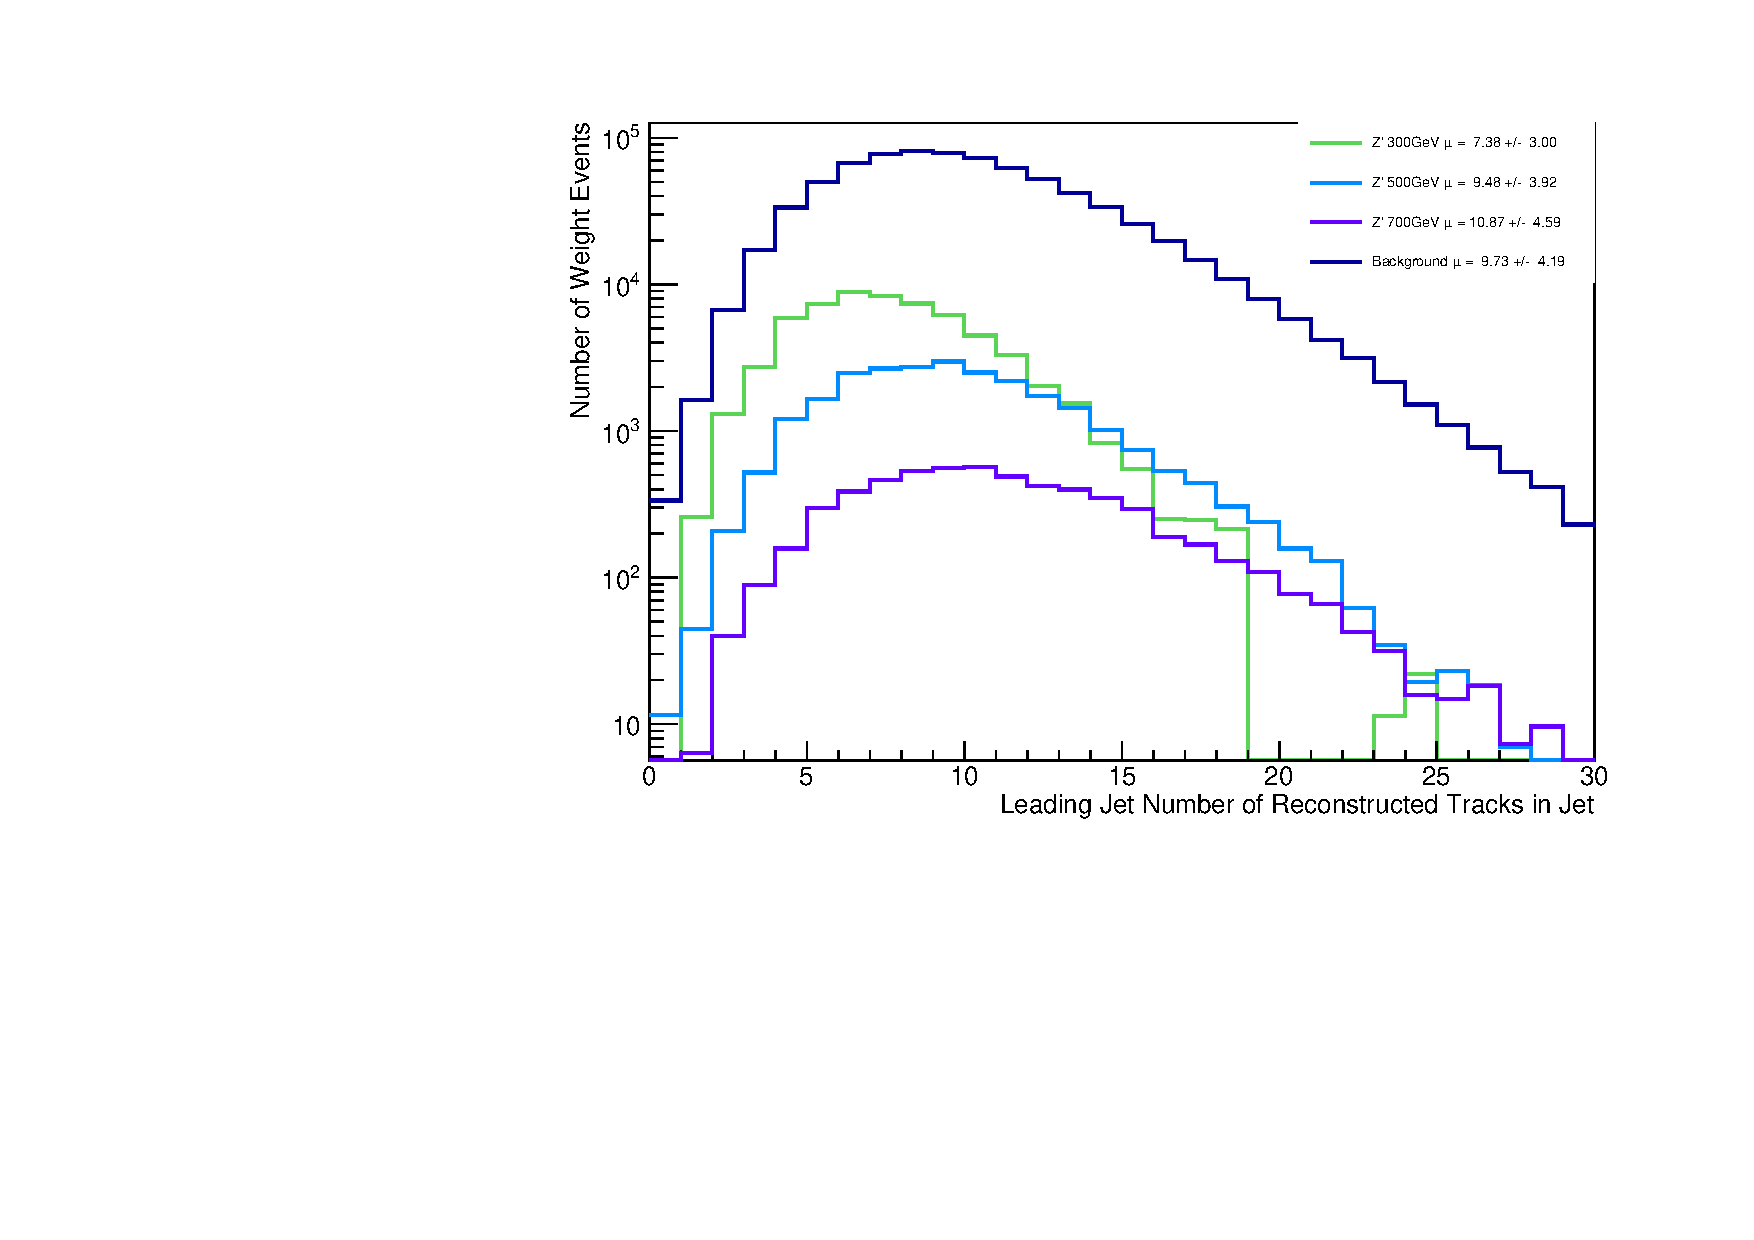
\includegraphics[width=0.45\hsize]{figures/QGT/sigWJ1_nTrk_Pass_Res_GGF_WW_SR.pdf}
 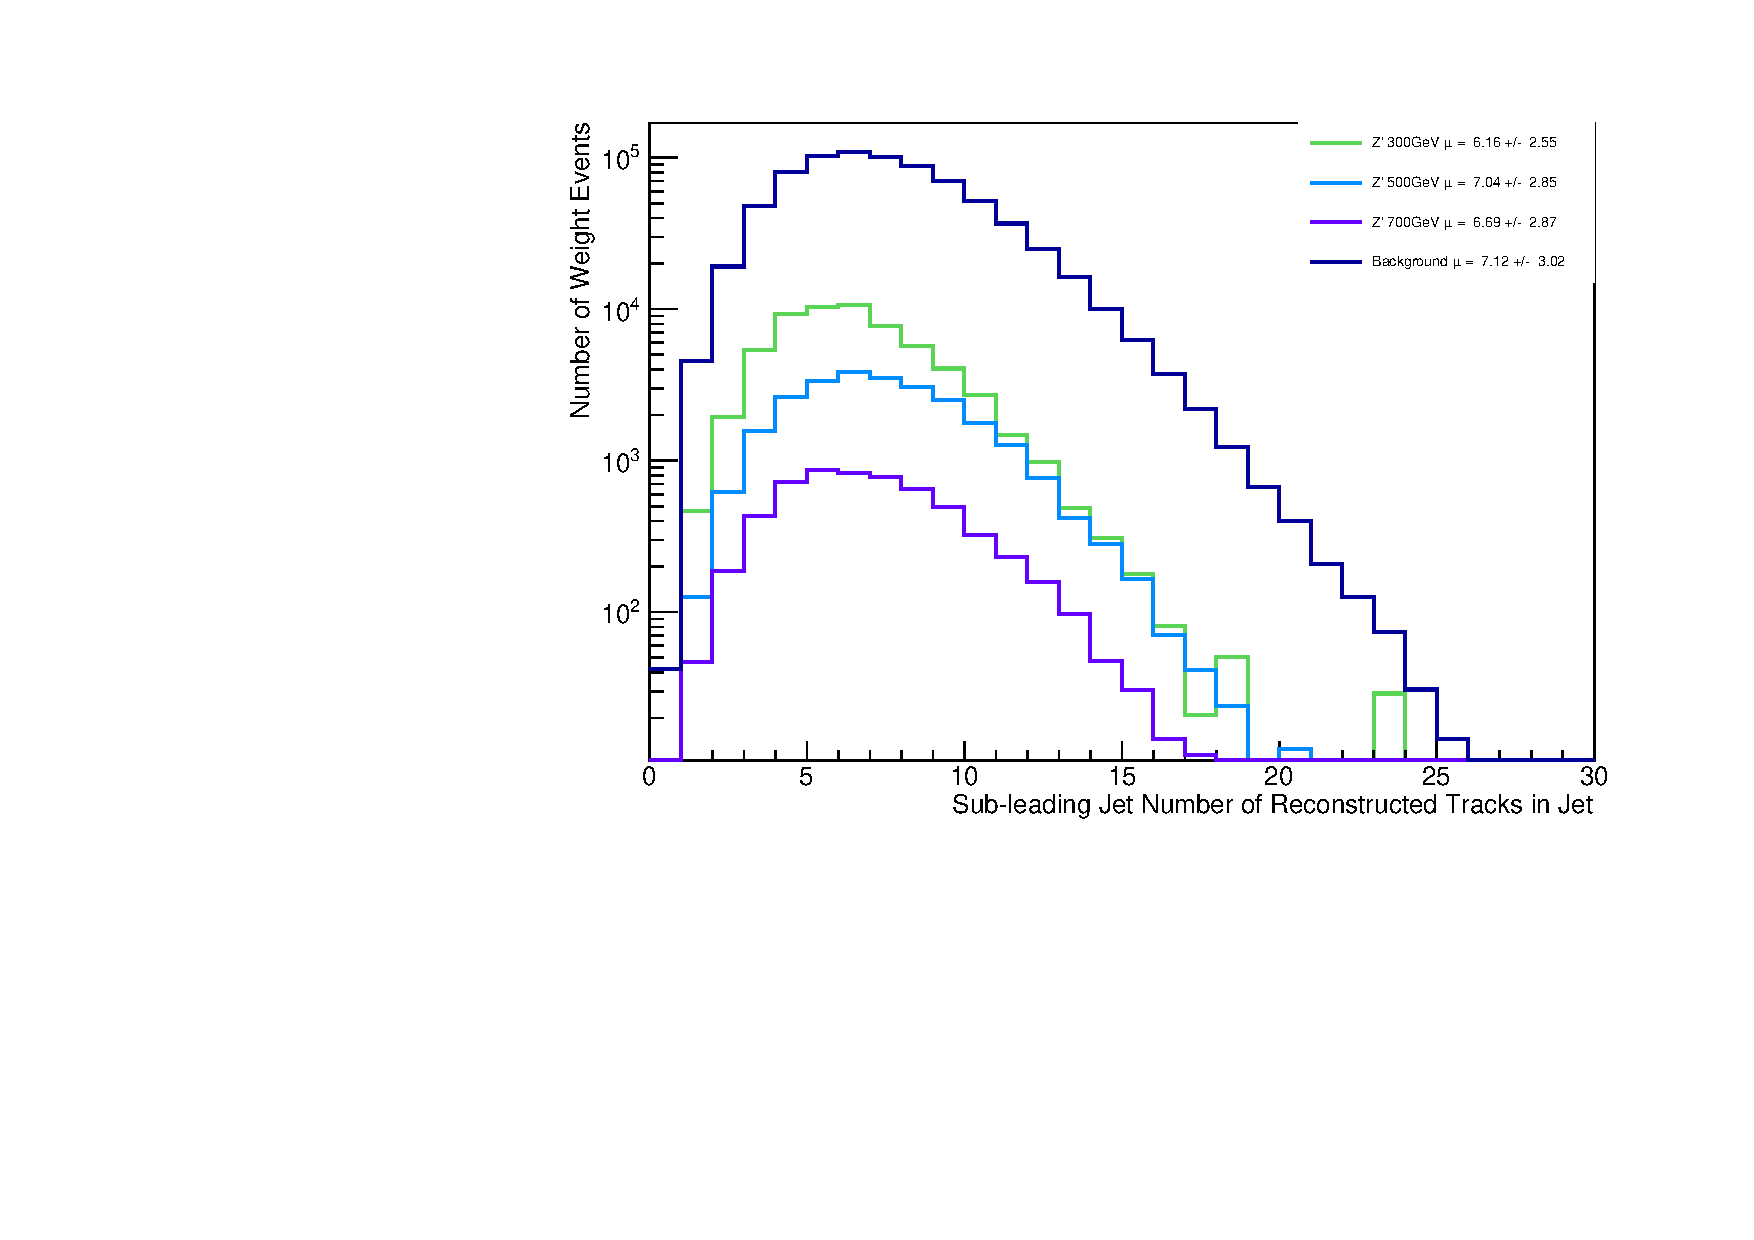
\includegraphics[width=0.45\hsize]{figures/QGT/sigWJ2_nTrk_Pass_Res_GGF_WW_SR.pdf}
  \caption{The number of tracks in small-R jets in events passing the Resolved GGF WW Signal Region selections for the (a) Leading (b) Sub-Leading jets. These distributions are shown for 300, 500, and 700GeV Z' signals and the background.}
  \label{fig:diag_ntrk}
\end{figure}
\FloatBarrier


\begin{figure}[h!]
  \centering
  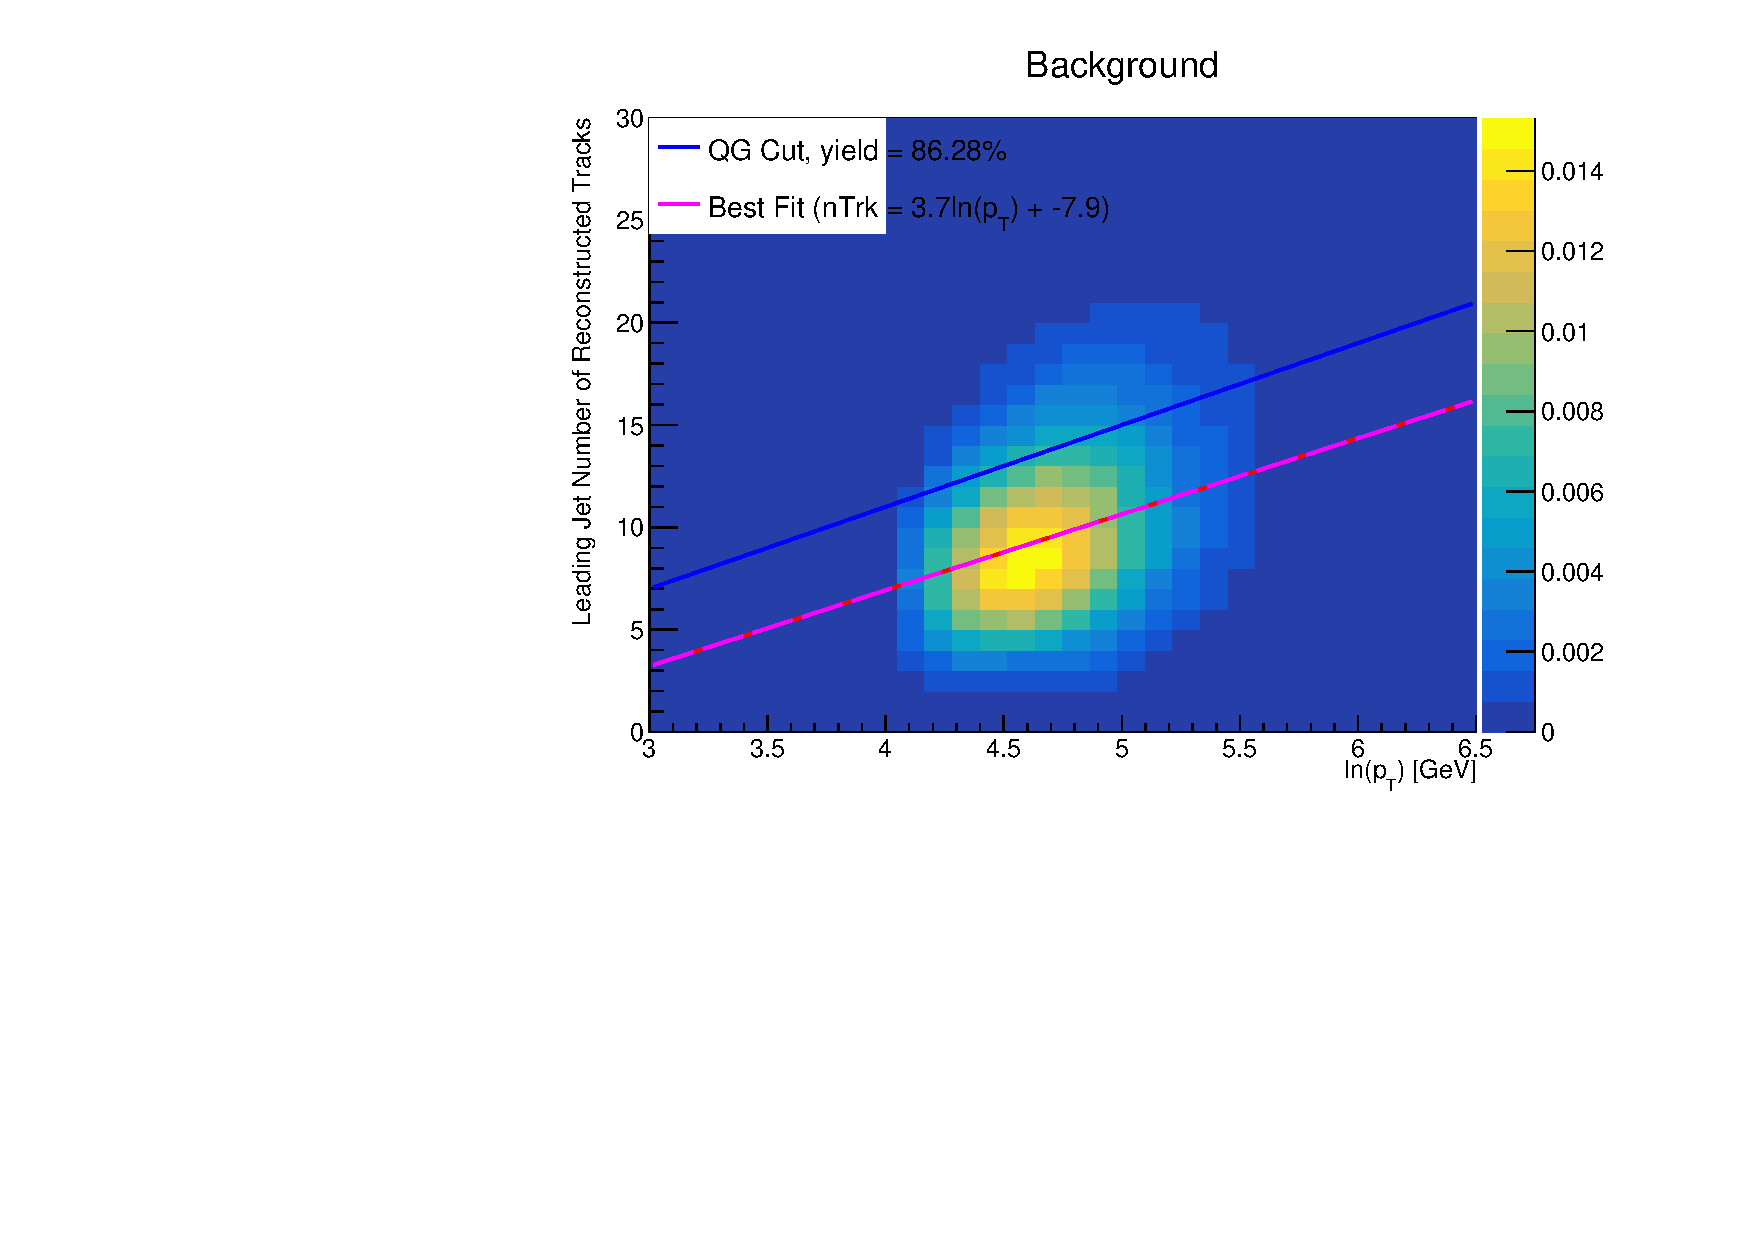
\includegraphics[width=0.45\hsize]{figures/QGT/allbkg-ade_Pass_Res_GGF_WW_SR_sigWJ1_nTrk.pdf}
 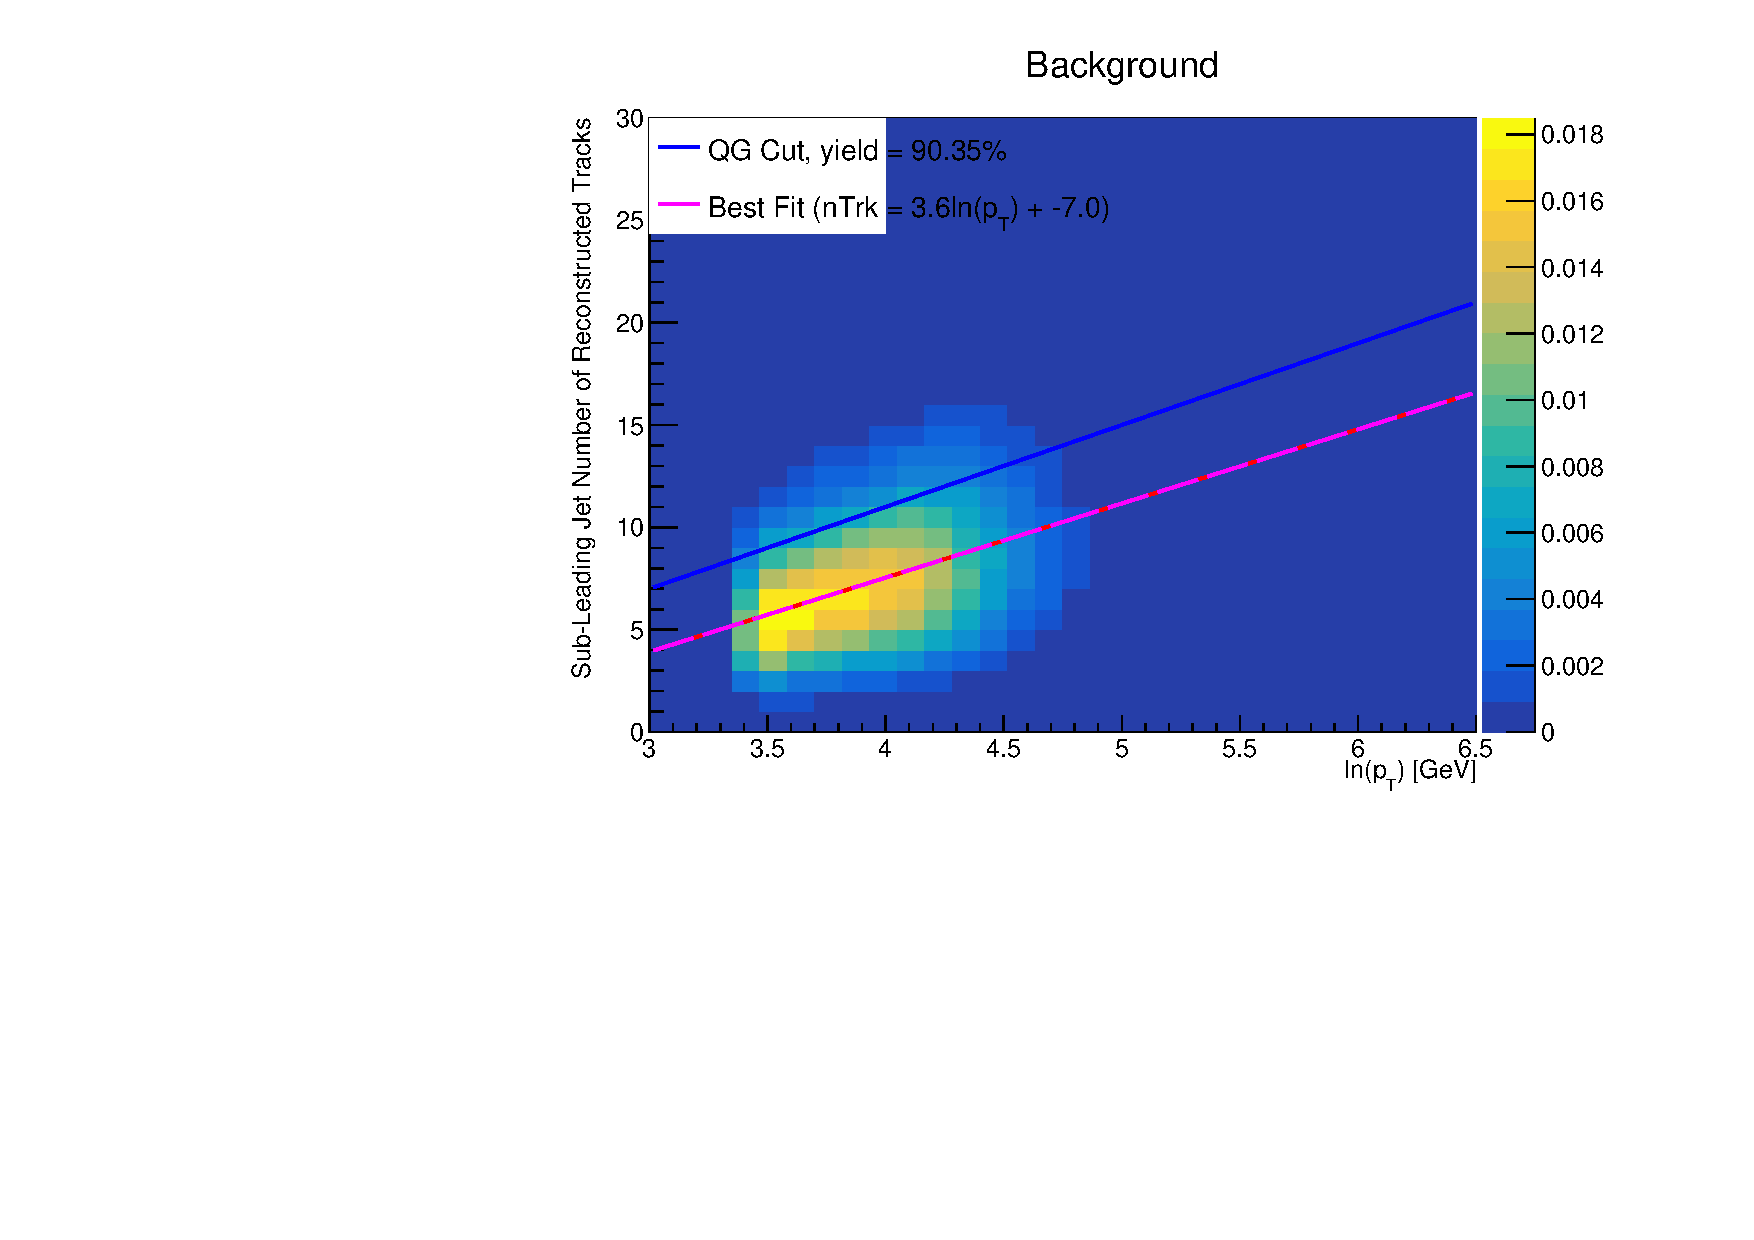
\includegraphics[width=0.45\hsize]{figures/QGT/allbkg-ade_Pass_Res_GGF_WW_SR_sigWJ2_nTrk.pdf}
  \caption{The number of tracks in background small-R jets in events passing the Resolved GGF WW Signal region selection vs. $ln(p_{T})$ for (a)Leading (b) Sub-Leading jets. The best fit line for the distribution is also shown, as well as the percentage of jets that pass a cut of number of tracks $< 4\times ln(p_{T}) -5$. Note the number of total entries in these plots has been normalized to one.}
  \label{fig:bkg_heatmap}
\end{figure}
\FloatBarrier


\begin{figure}[h!]
  \centering
  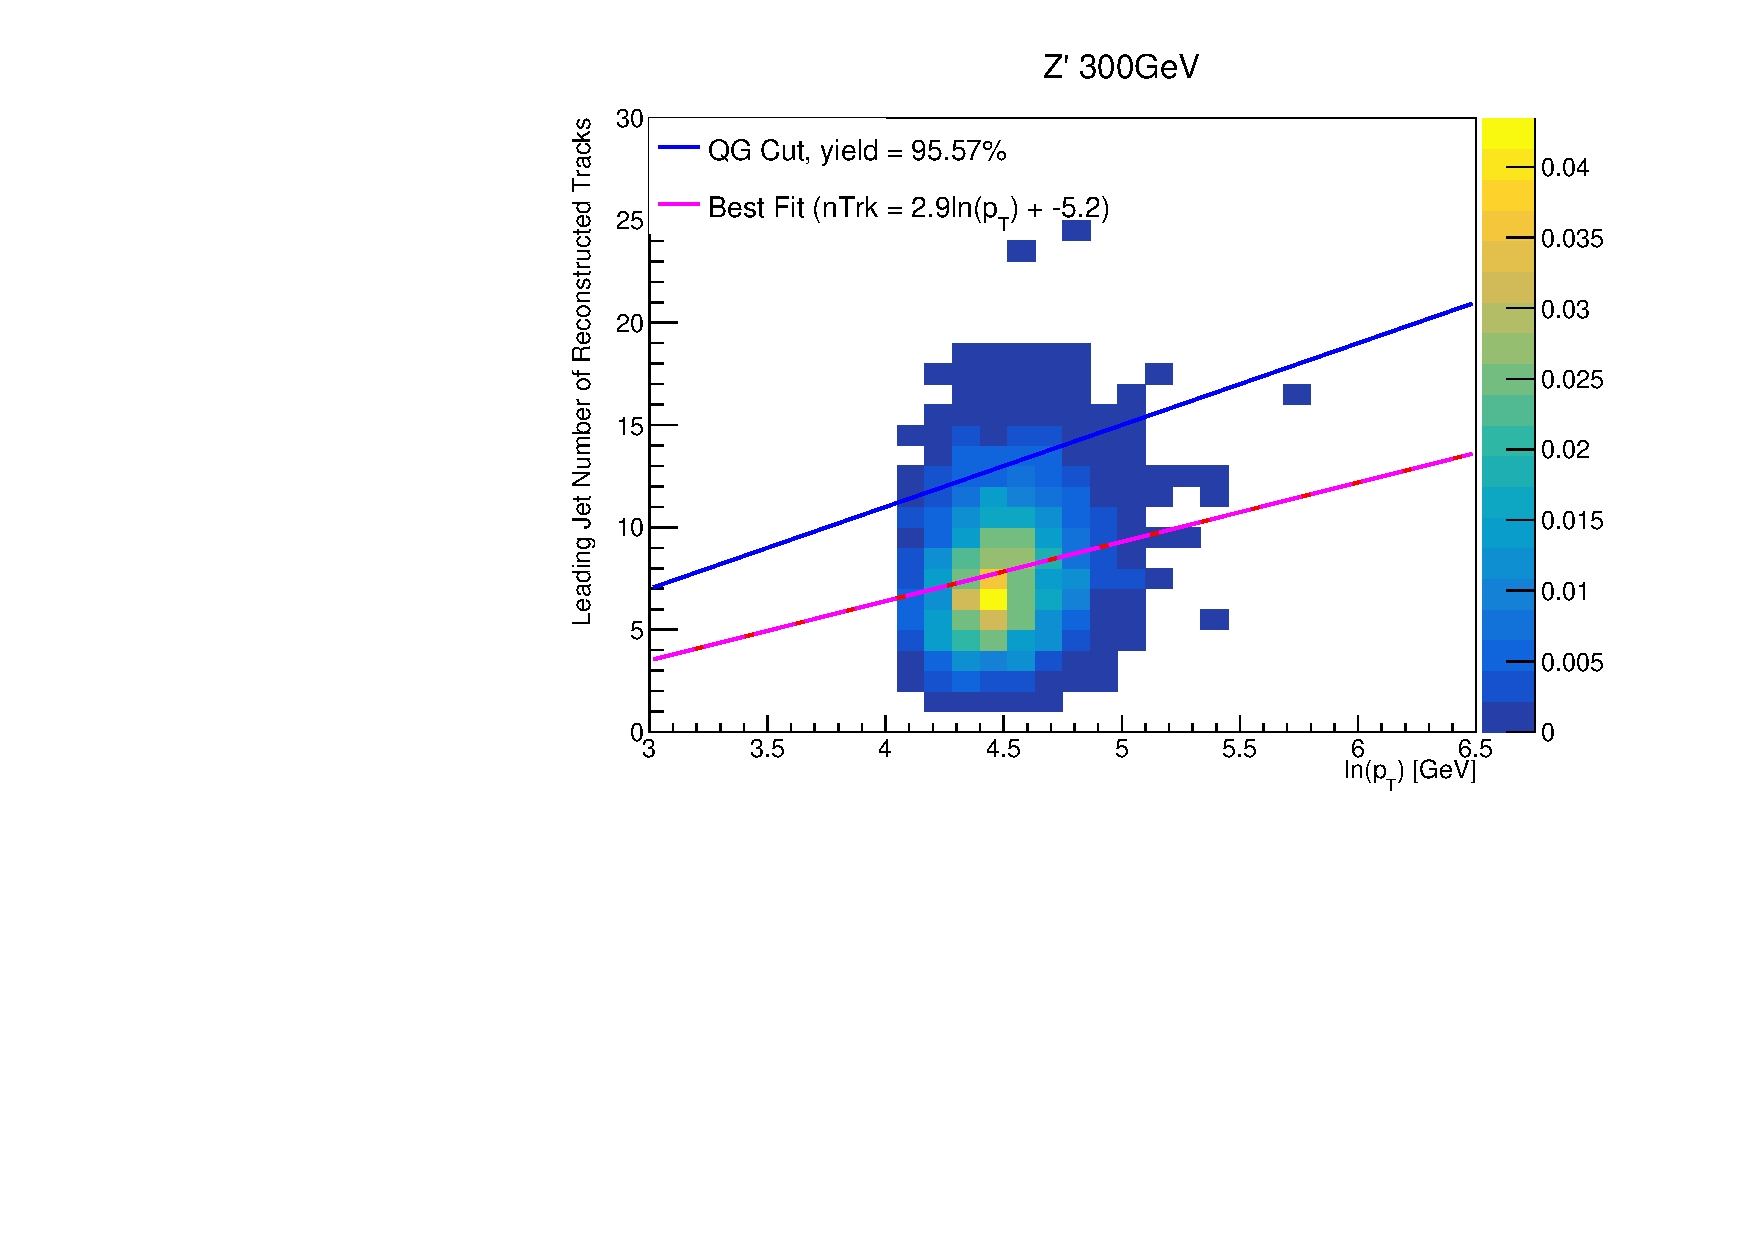
\includegraphics[width=0.45\hsize]{figures/QGT/HVTWW_300_1lep_Pass_Res_GGF_WW_SR_sigWJ1_nTrk.pdf}
 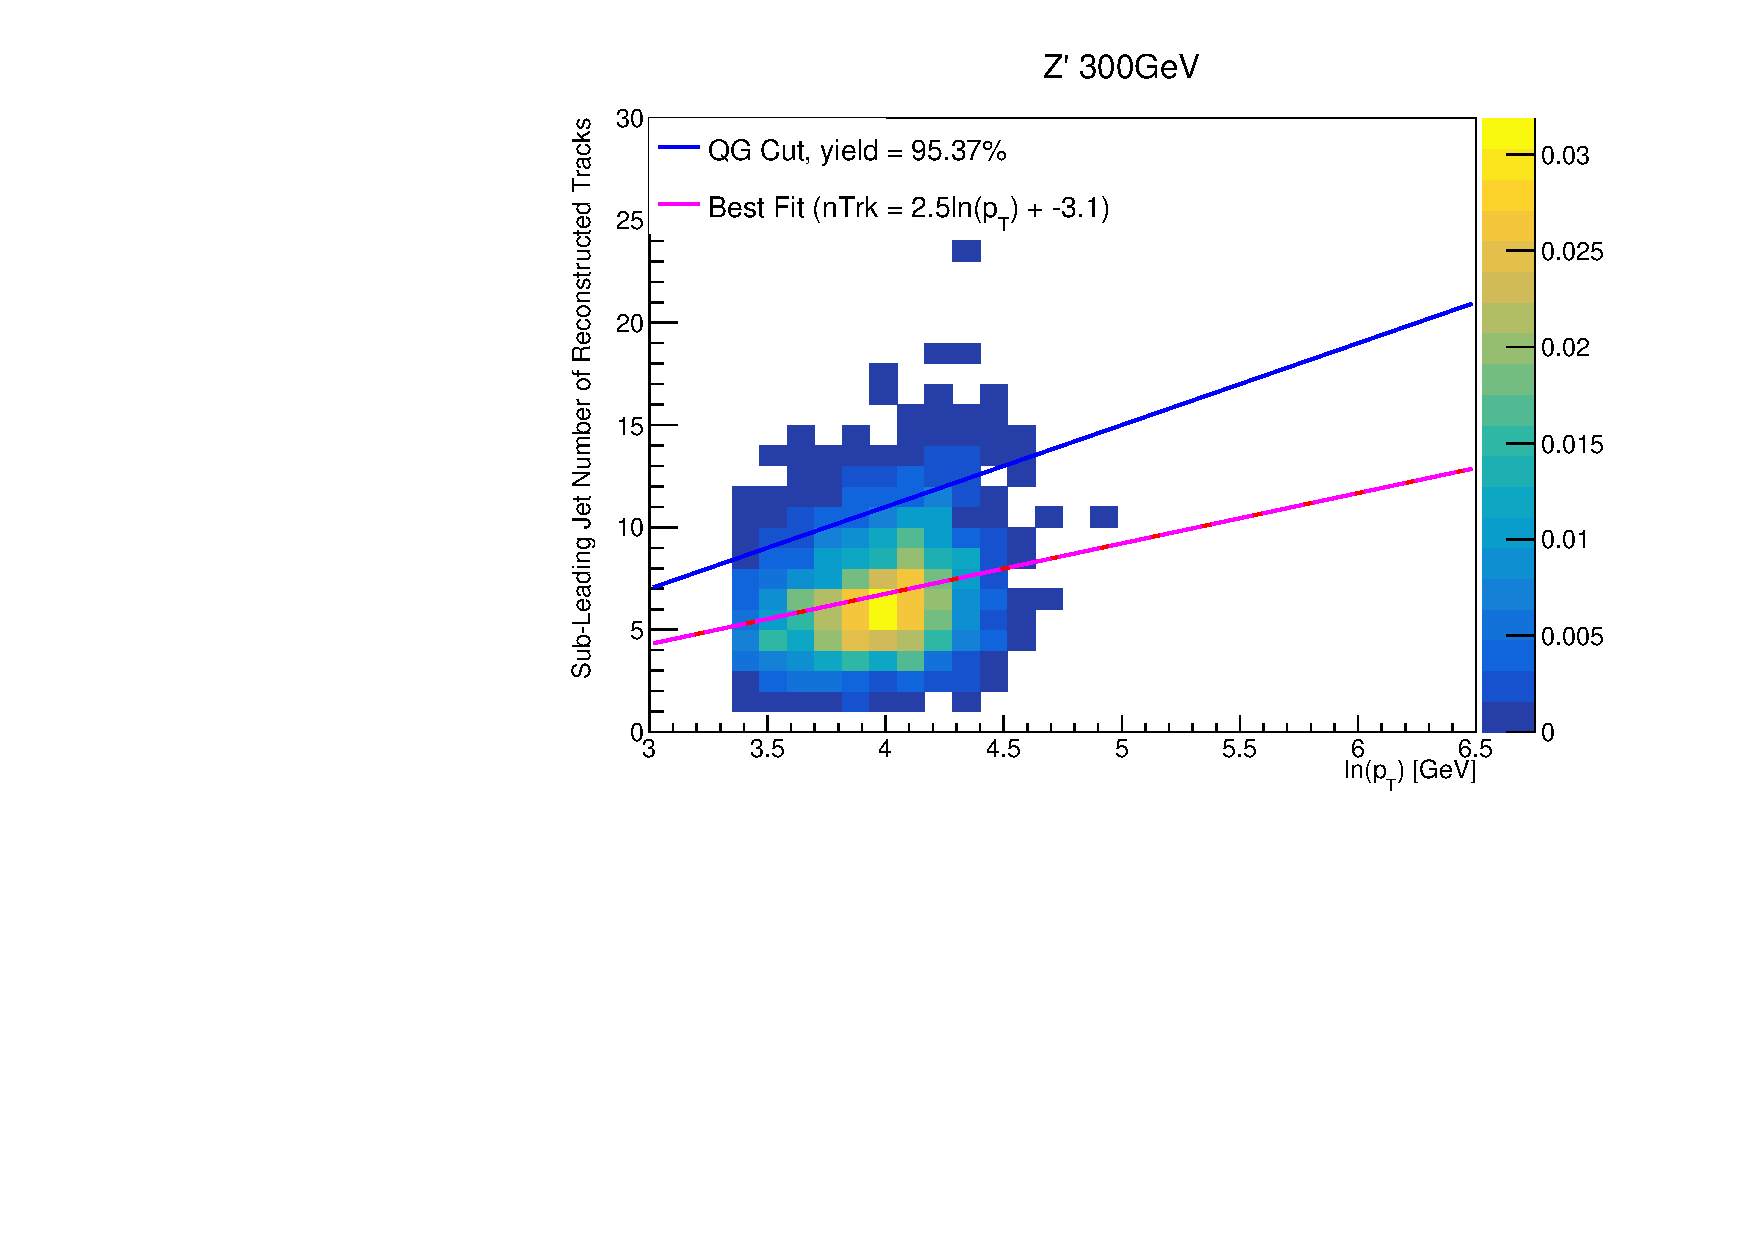
\includegraphics[width=0.45\hsize]{figures/QGT/HVTWW_300_1lep_Pass_Res_GGF_WW_SR_sigWJ2_nTrk.pdf}
  \caption{The number of tracks in small-R jets in 300GeV Z' events passing the Resolved GGF WW Signal region selection vs. $ln(p_{T})$ for (a)Leading (b) Sub-Leading jets. The best fit line for the distribution is also shown, as well as the percentage of jets that pass a cut of number of tracks $< 4\times ln(p_{T}) -5$.Note the number of total entries in these plots has been normalized to one.}
  \label{fig:sig300_heatmap}
\end{figure}
\FloatBarrier


\begin{figure}[h!]
  \centering
  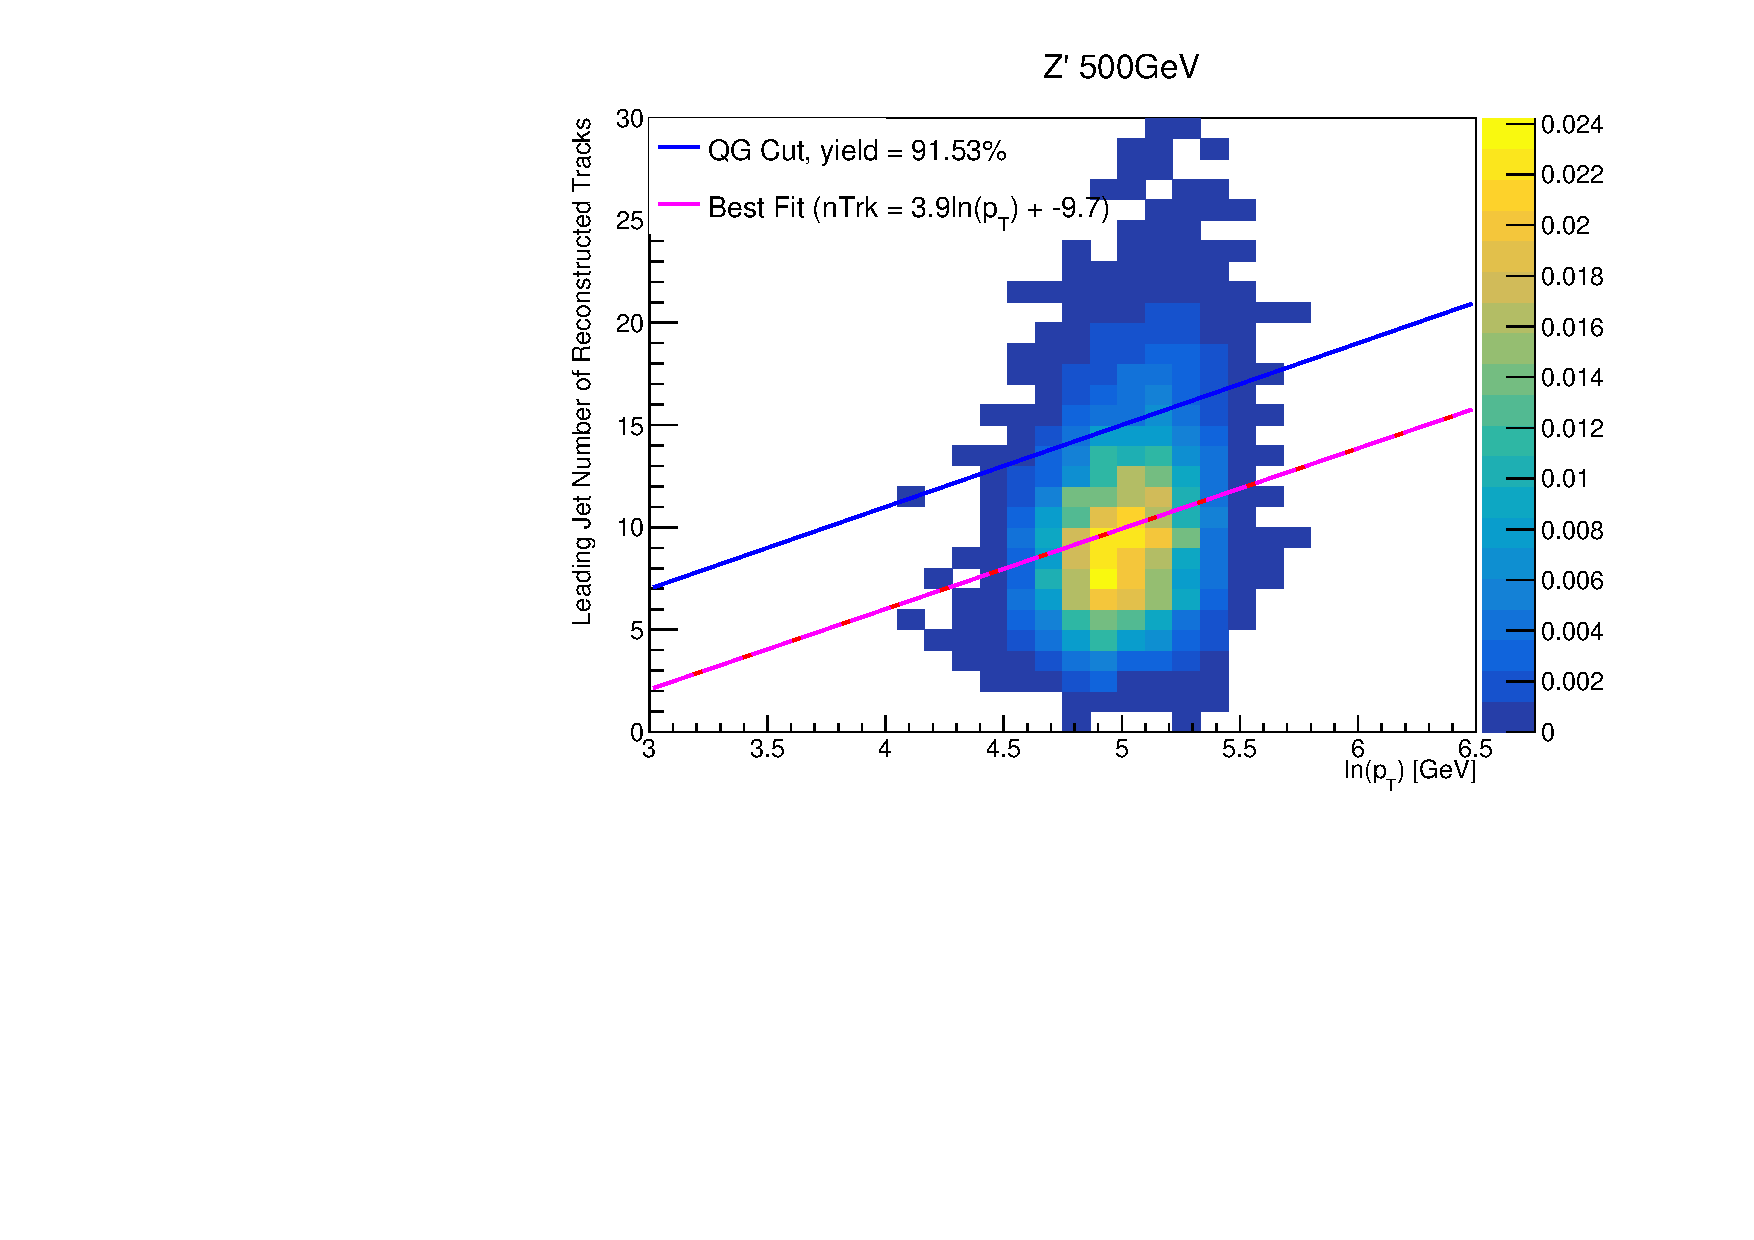
\includegraphics[width=0.45\hsize]{figures/QGT/HVTWW_500_1lep_Pass_Res_GGF_WW_SR_sigWJ1_nTrk.pdf}
 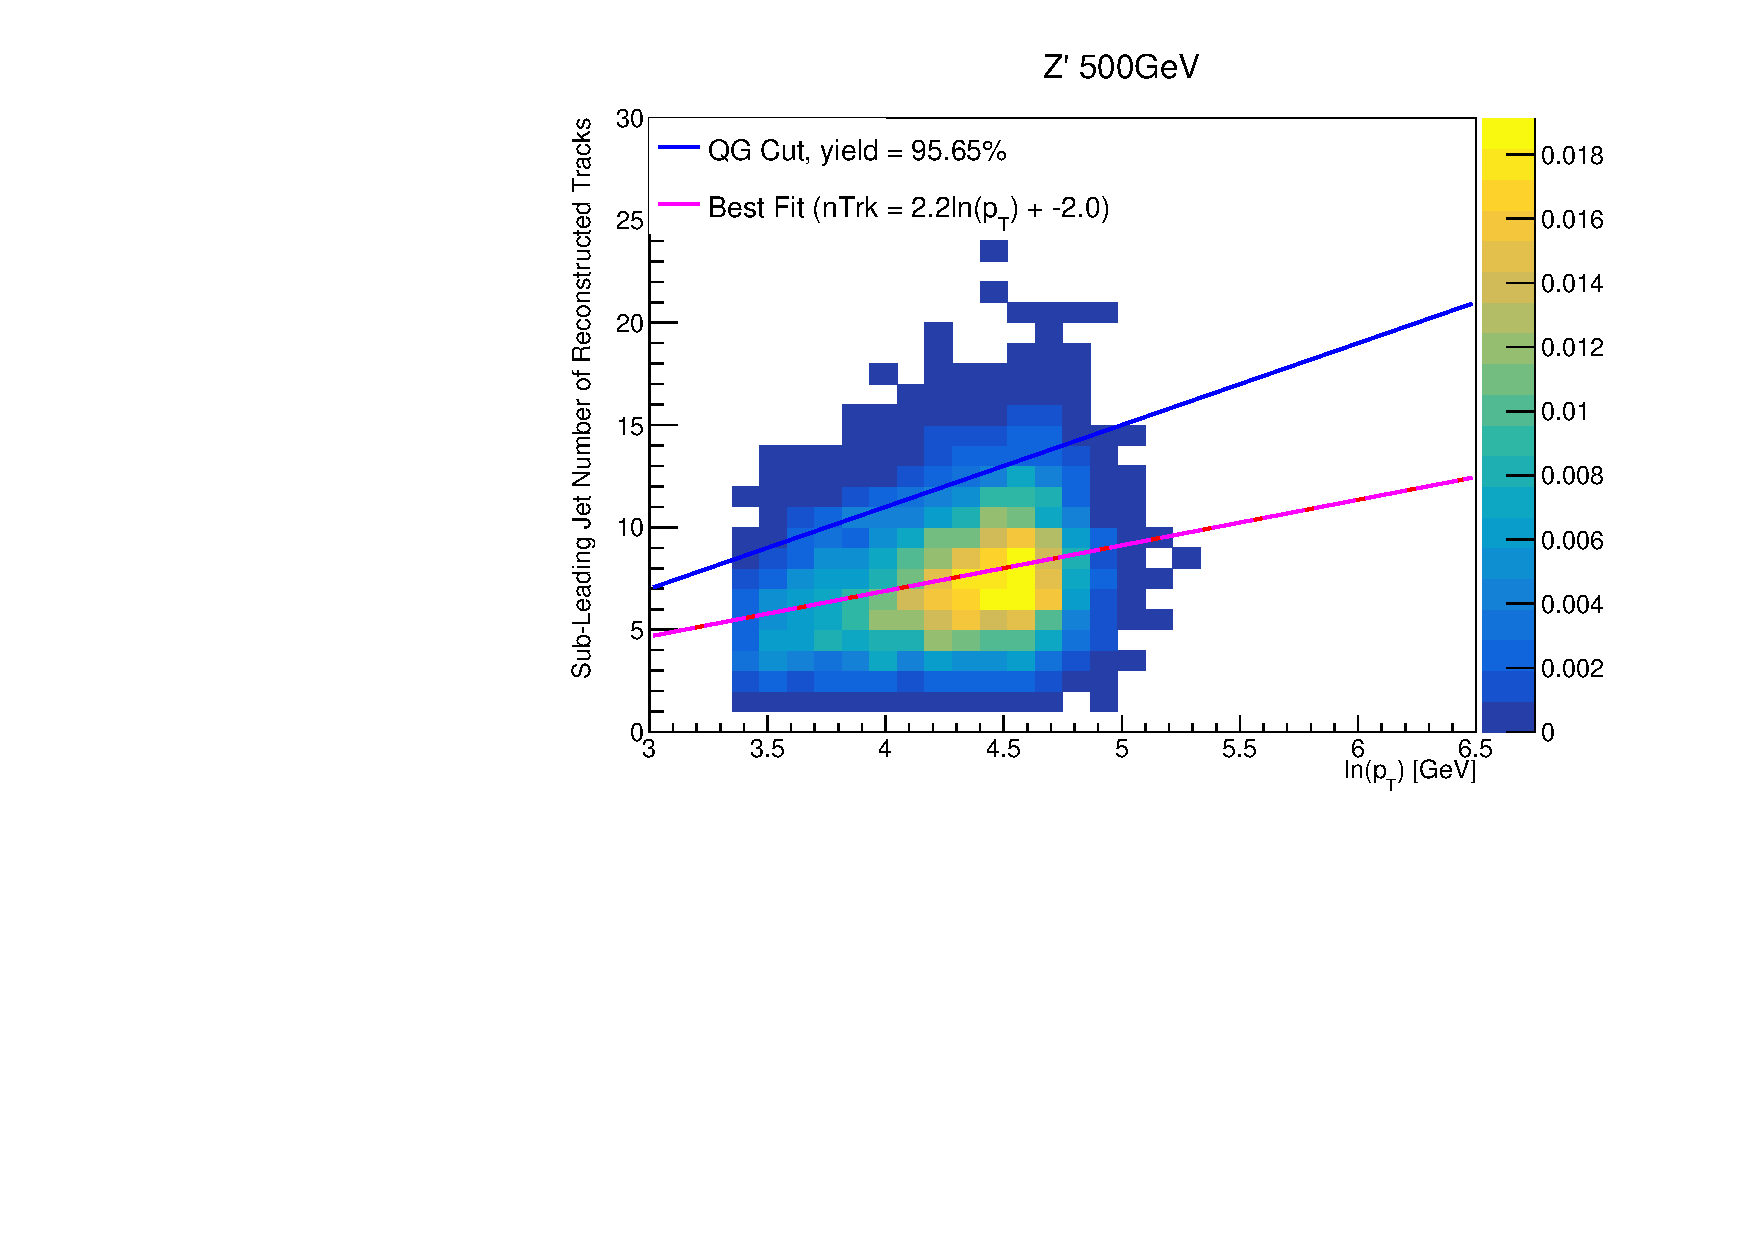
\includegraphics[width=0.45\hsize]{figures/QGT/HVTWW_500_1lep_Pass_Res_GGF_WW_SR_sigWJ2_nTrk.pdf}
  \caption{The number of tracks in small-R jets in 500GeV Z' events passing the Resolved GGF WW Signal region selection vs. $ln(p_{T})$ for (a)Leading (b) Sub-Leading jets. The best fit line for the distribution is also shown, as well as the percentage of jets that pass a cut of number of tracks $< 4\times ln(p_{T}) -5$.Note the number of total entries in these plots has been normalized to one.}
  \label{fig:sig500_heatmap}
\end{figure}
\FloatBarrier


\begin{figure}[h!]
  \centering
  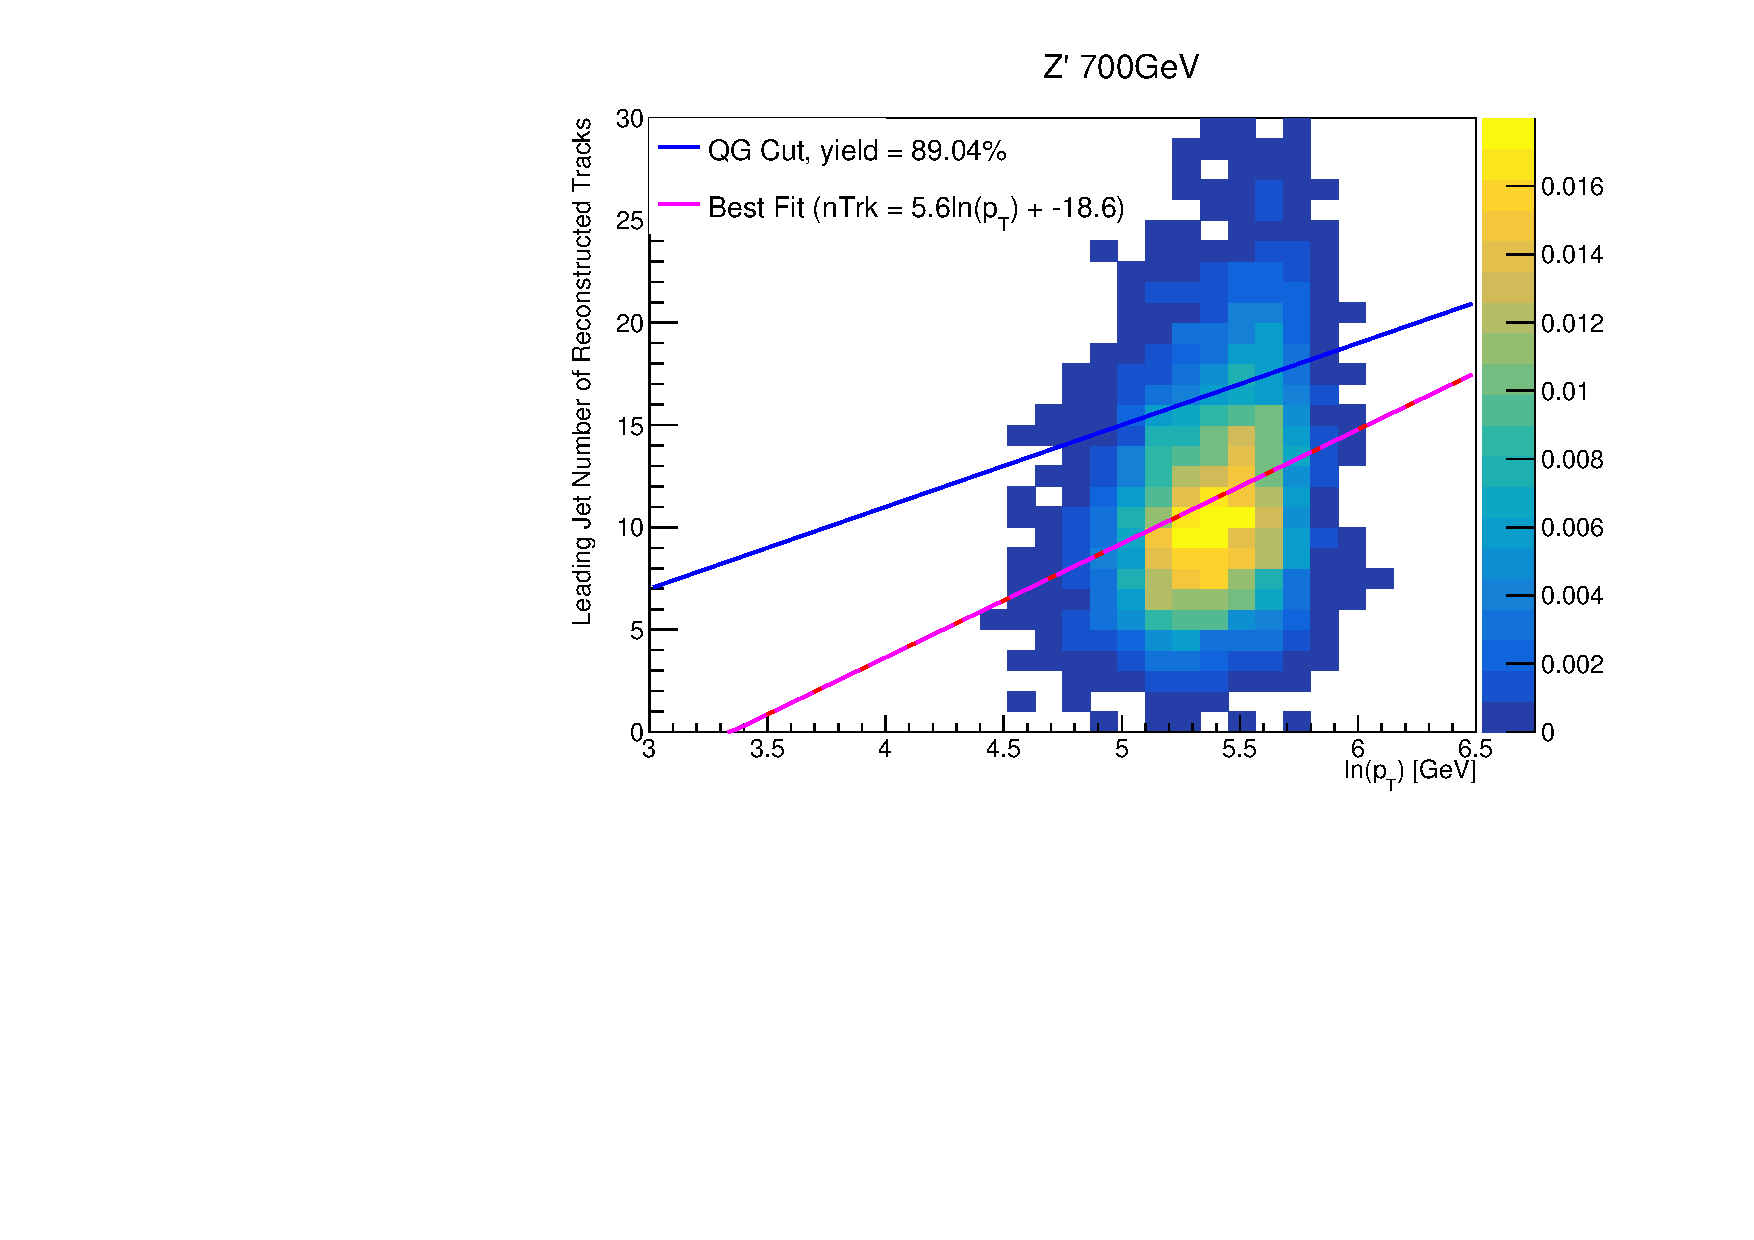
\includegraphics[width=0.45\hsize]{figures/QGT/HVTWW_700_1lep_Pass_Res_GGF_WW_SR_sigWJ1_nTrk.pdf}
 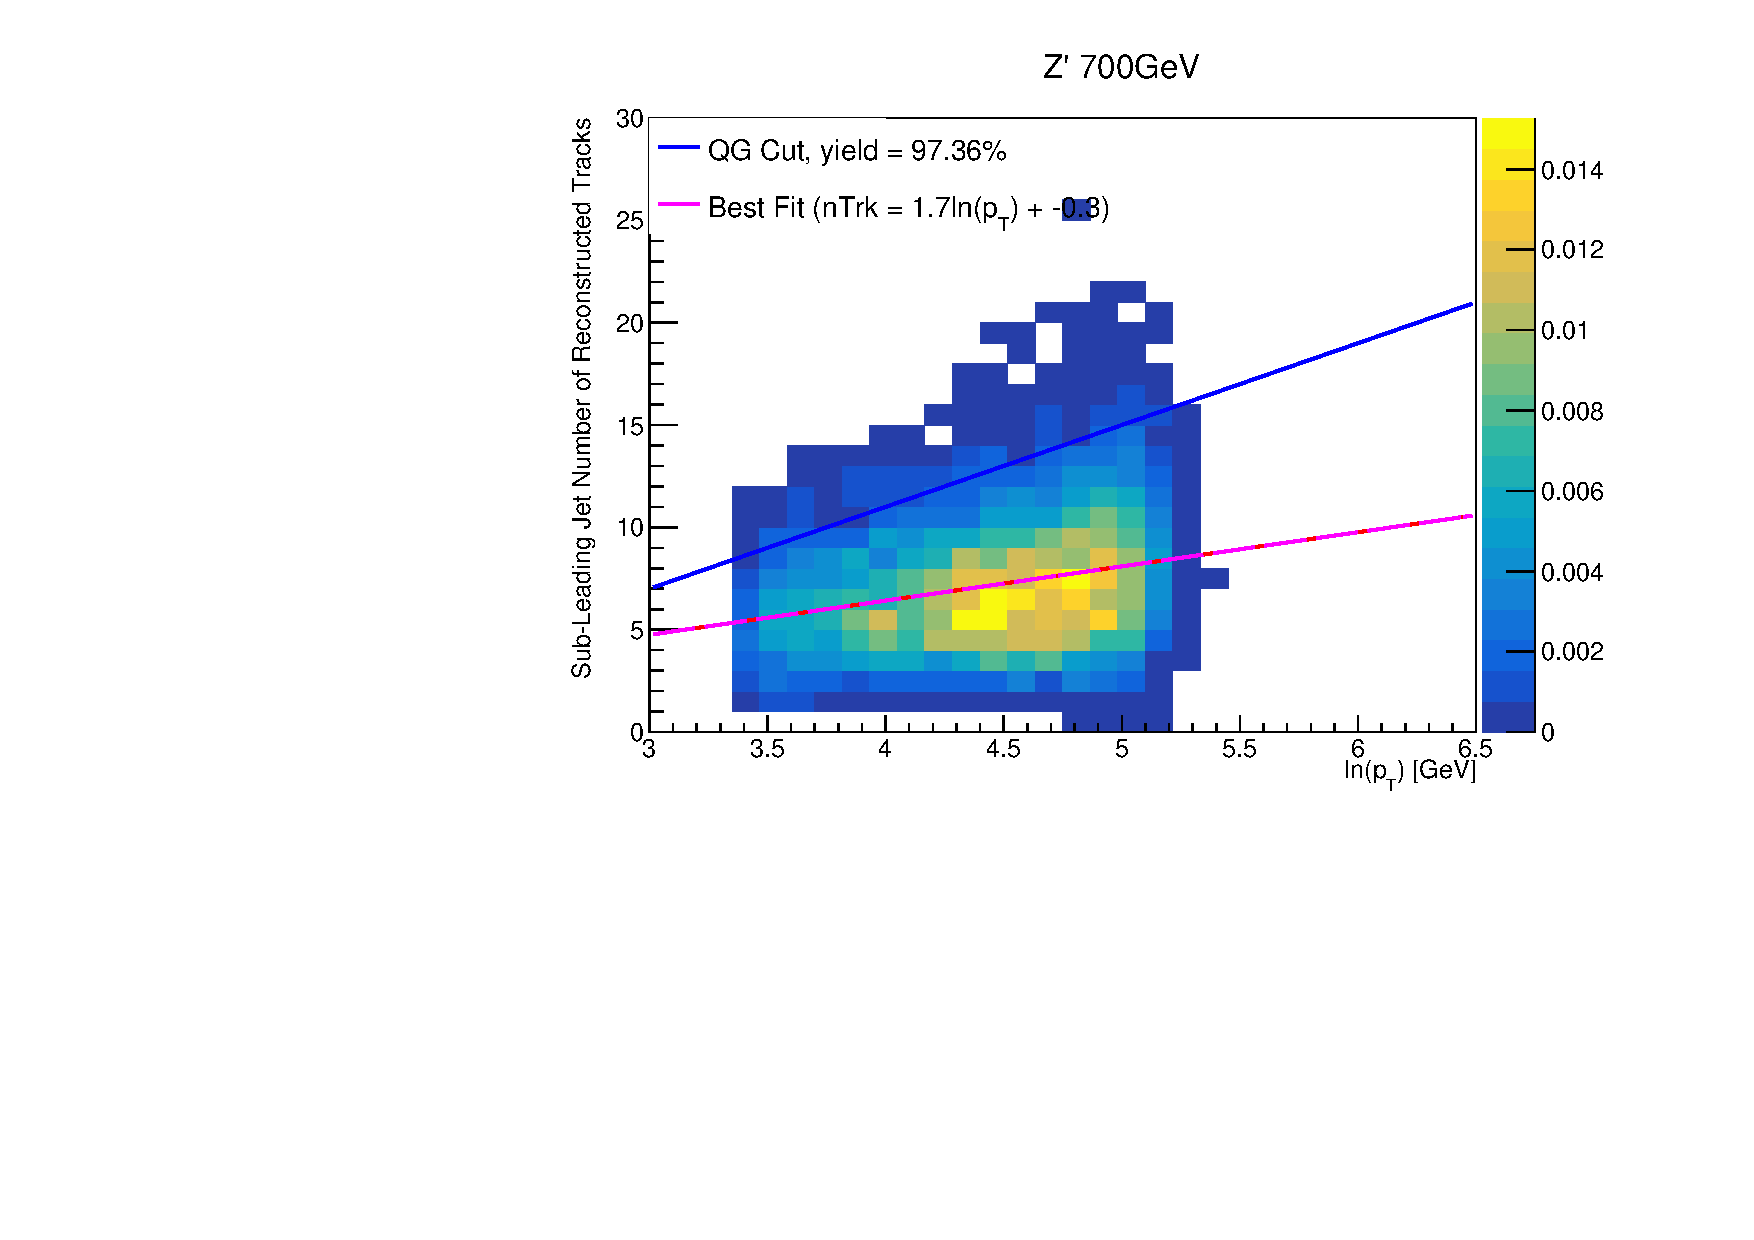
\includegraphics[width=0.45\hsize]{figures/QGT/HVTWW_700_1lep_Pass_Res_GGF_WW_SR_sigWJ2_nTrk.pdf}
  \caption{The number of tracks in small-R jets in 700GeV Z' events passing the Resolved GGF WW Signal region selection vs. $ln(p_{T})$ for (a)Leading (b) Sub-Leading jets. The best fit line for the distribution is also shown, as well as the percentage of jets that pass a cut of number of tracks $< 4\times ln(p_{T}) -5$.Note the number of total entries in these plots has been normalized to one.}
  \label{fig:sig700_heatmap}
\end{figure}
\FloatBarrier


\begin{table}
\begin{tabular}{|l|c|c|c|}
\hline
Sample & Best Fit Slope & Best Fit Intercept & QG Tag Yield \\\hline
Backgrounds & 3.7 & -7.9 & 86\% \\\hline
HVT $Z'$ 300 GeV &  2.9 & -5.2 & 95\% \\\hline
HVT $Z'$ 500 GeV & 3.9 & -9.7 & 92\% \\\hline
\end{tabular}
\caption{This table shows the best fit slope and intercept for the 2-d distribution of number of tracks vs. jet $\ln(p_{T})$ for the leading jet in the background and HVT $Z'$ samples. The tagging efficiency is shown for the 90\% working point in the last column. The background jets contain more gluons than the signal jets. Consequently, the best fit line for the background predicts larger values of the number of tracks in jets for the background than the considered signals.}
\label{tbl:hvtwzvbf_norm}
\end{table}

\begin{figure}[h!]
  \centering
  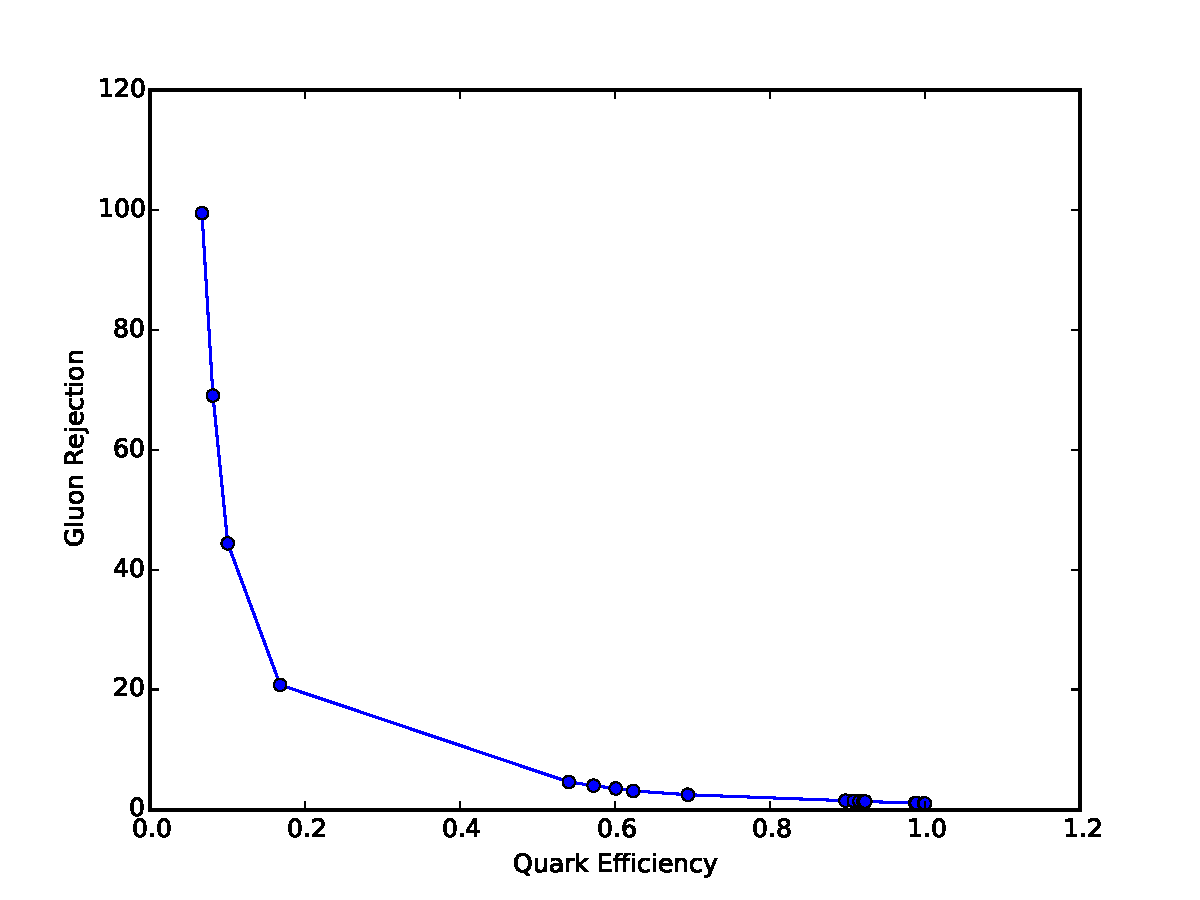
\includegraphics[width=\hsize]{figures/QGT/finalroc.pdf}
  \caption{ROC Curve for Quark and Gluon Tagging with a cut on the number of tracks that depends on the $ln(p_{T})$.}
  \label{fig:quark_gluon_roc}
\end{figure}
\FloatBarrier


\begin{figure}[h!]
  \centering
  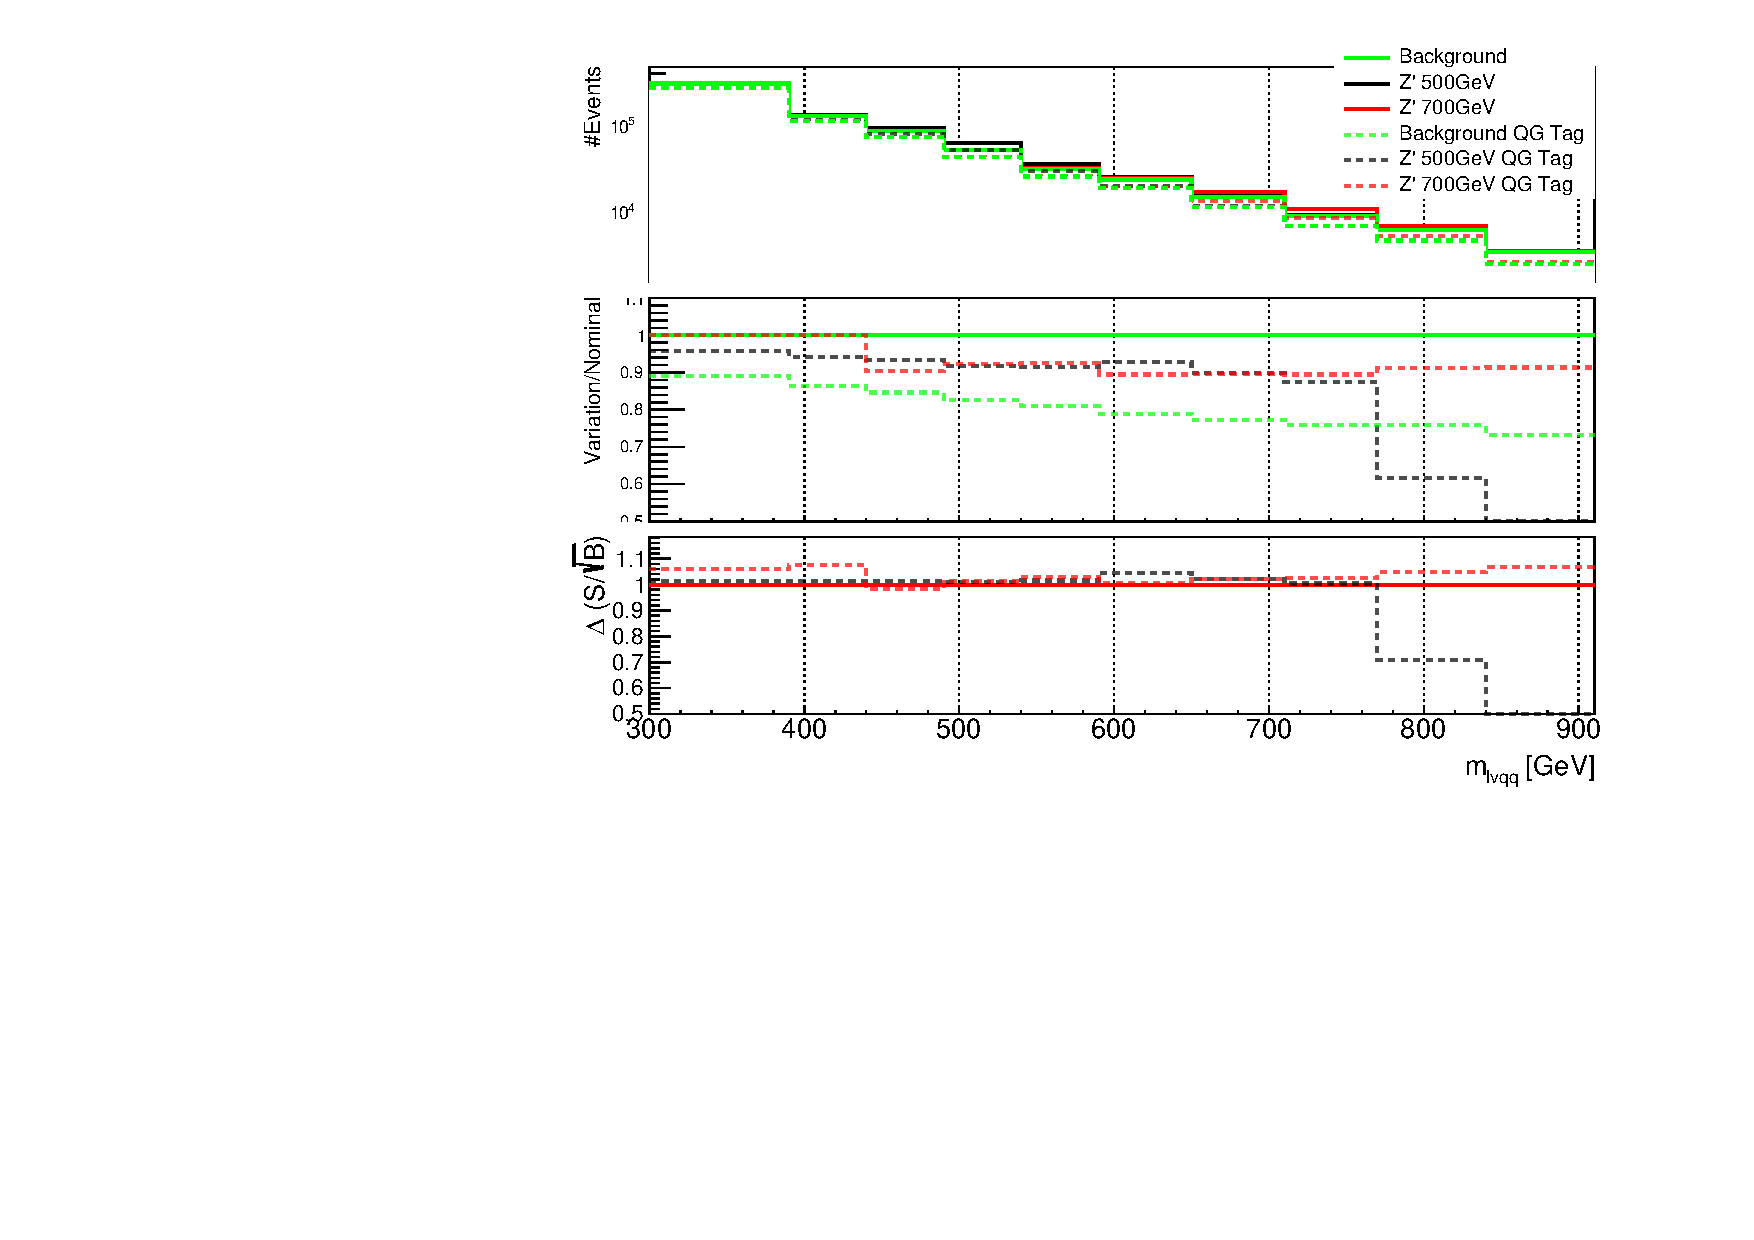
\includegraphics[width=\hsize]{figures/QGT/s_root_b_recotag.pdf}
  \caption{The top panel shows the distribution of $m_{lvqq}$ with and without quark gluon tagging. The middle panel shows the ratio of the signals and backgrounds with and without quark gluon tagging. The bottom panel shows the change in $S/\sqrt{B}$ with quark gluon tagging.}
  \label{fig:qg_s_root_b}
\end{figure}
\FloatBarrier


\pagebreak
\pagebreak
\pagebreak
\chapter{$n_{trk}$ Calibration}
The number of tracks in jets depends on modeling and experimental systematics. Consequently, the efficiency of a quark-gluon tagger based on the number of tracks in jets would have associated uncertainties. In the context of the resonance search discussed, these uncertainties would be treated as systematics that impact the $m_{WV}$ distributions that are used for discovery tests.

Modeling uncertainties are obtained by assessing PDF and ME uncertainties on the number of charged particles in particle-level jets in dijet events. The number of charged particles as a function of jet $p_{T}$  is calculated using an Iterative Bayesian (IB) technique [cite paper].

This measurement (\cite{Unfolding}) uses the ATLAS 2012 pp collision dataset, corresponding to 20.3/fb at center-of-mass energy $\sqrt{s}=8$TeV. The number of charged constituents depends on fragmentation modeling and matrix elements, which do not depend on s. For this reason, it is safe to use these uncertainties for sqrt(s)=13TeV. Monte Carlo (MC) samples are used to determine the response matrix. The MC sample is a dijet sample generated with Pythia 8.175 using CT10 PDF and AU2 tune.  The anti-$k_{T}$ algorithm is used to cluster jets with a radius parameter R = 0.4. Jets are required to have $|\eta| < 2.1$. Tracks in jets are required to have $p_{T}>500MeV$, $|\eta|<2.5$, track-fit $\chi^{2} < 3.0$ and originate from the primary vertex. Matching tracks to jets is accomplished using ghost-association [cite]. In this technique, jets are re-clustered with the track collection augmented with "ghost" versions of tracks.  These "ghosts" tracks have the same direction as their parent track, but infinitesimal track $p_{T}$. This insures meta-jet properties (e.g. $\eta$, $p_{T}$, etc) are unchanged. A track is matched to a jet if it's ghost version remains in the jet after re-clustering. Further details of the data, object, and event selection may be found in [cite 35].

To select dijet topologies events are required to have at least two jets with $p_{T} > 50GeV$ that are relatively well-balanced ($p_{T}^{lead}/p_{T}^{sub-lead} < 1.5$). 

In the IB technique, the prior distribution and number of iterations are the inputs [cite Bayesian paper]. The IB response matrix connects number of charged particles to the number of tracks in jets determined using the simulated samples. This response matrix is used to unfold data to extract the $n_{c}$. Before applying the response matrix a fake factor is applied. This accounts for jets that pass detector level selections, but not particle level selections. Following this, the IB method iteratively applies the response matrix using the nominal Pythia 8.175 sample as a prior. The number of IB iterations is chosen to minimize unfolding bias and statistical fluctuations. For this measurement four iterations was found to be optimal by minimizing the unfolding bias from pseudodata simulated with Herwig++ with a prior from Pythia 8 AU2. Finally, the inefficiency factor is applied to account for events passing particle level selection but not detector level, yielding the unfolded nCharged distribution.
 
This process is prone to three main sources of bias: response matrix, correction factor, and unfolding procedure uncertainties. The response matrix is sensitive to experimental uncertainties impacting jet track reconstruction and calorimeter jet $p_{T}$. Correction factors are also sensitive to experimental uncertainties (e.g. JES) as such uncertainties modify detector level acceptance. Sensitivity to particle level acceptance is calculated by comparing Pythia and Herwig. Finally, the bias from the IB prior choice is determined by reweighting the particle-level spectrum, so the simulated detector level spectrum more closely matches the uncorrected data. Unfolding this modified detector-level simulation and comparing it to the re-weighted particle-level spectrum indicates bias from the prior distribution choice.

A summary of all the systematic uncertainties associated with this unfolding may be found in [ref paper]. Total uncertainties are < 7\% for the number of charged particles in jets. The unfolded distribution of the nCharged in jets from data are further analyzed to extract the quark and gluon nCharged distributions. In dijet events, the jet with a larger $\eta$ is more energetic and therefore more likely to be a quark. This is due to the quarks in protons generally having a larger fraction of the total momentum of the proton constituents. The more central jet is more likely to be a gluon-initiated jet. This correlation between jet $\eta$ and flavor may then be used to extract nCharged in $p_{T}$ bins using:

\begin{equation}
<n_{c}^{f}> = f_{q}^{f}<n_{c}^{q}> + f^{f}_{g}<n_{c}^{g}>
\end{equation}
\begin{equation}
<n_{c}^{c}> = f_{q}^{c}<n_{c}^{q}> + f^{c}_{g}<n_{c}^{g}> 
\end{equation}


In this equation the f and c subscripts denote the more forward and central jets, respectively. The q and g subscripts denote quark and gluon. The fraction of more forward jets that are say gluons is denoted by $f_{g}^{f}$. The other relevant jet fractions are denoted with the same naming scheme. Finally, $<n_{c}>$ is the average number of charged particles in a jet in a given $p_{T}$ bin. To show that Eq. ~\eqref{QG_extraction} may be used to extract quark and gluon $n_{c}$ distributions the extracted distributions are compared to $n_{c}$ distributions determined using the jet flavor in simulation. Figure [add figure natasha] shows that the extracted and true distributions differ by < 1\% over the $p_{T}$ range probed for this study. Moreover, this implies that $n_{c}$ depends only on the flavor of the initiating parton and jet $p_{T}$. 

These extracted distributions are prone to PDF and ME biases. The bias from the choice of the CT10 PDF for the Pythia sample is accounted for by comparing quark/gluon fractions for the nominal CT10 sample with its eigenvector variations. Comparing the quark/gluon fractions from Pythia 8 and Herwig++ quantify the uncertainity from the ME calculation. These uncertainities are added in quadrature with the unfolding uncertainity to give the total modelling uncertainity on the extracted $n_{c}$ distribution. This is shown in Figure~\ref{fig:extracted_qg}.

To apply these uncertainities in $n_{c}$ distributions in data, per-jet event weights are associated with each uncertainity according to:

\begin{equation}
w_{i}(n_{c}) = \frac{P(n_{c}|<n_{c}> \pm \sigma^{i}_{n_{c}})} {P(n_{c}|<n_{c}>)}
\end{equation}

In Eq. ~\eqref{QG_uncer}, i denotes the uncertainty considered, P is the Poisson probability, and $\sigma^{i}_{n_{c}}$ represents the average impact of the uncertainity on $n_{c}$. 

%DETECTOR LEVEL UNCERTAINTIES 
%(mc16_13TeV.361020.Pythia8EvtGen_A14NNPDF23LO_jetjet_JZ0W.merge.DAOD_JETM1.e3569_s2997_r8903_r8906_p2996).


The previous uncertainties described accounted for modeling uncertainty associated with the number of charged particles in a jet. However, $n_{c}$ is not a measurable quantity. Instead the number of tracks in a jet is measured, which is a proxy for $n_{c}$. Therefore the uncertainties associated with the measurement of nTracks must also be considered (\cite{JetFrag}). These uncertainties were calculated using a Pythia 8 dijet sample with NNPDF 23 and Run 2 data. Track reconstruction efficiency and fake rates are the dominant sources of nTrack uncertainties. 

The track reconstruction efficiency is affected by the uncertainty of the description of the ID material in simulation and the modeling of charged-particle interactions with this material. These uncertainties are accounted for by varying the ID material by 5-25\% (dependent on the region of the detector considered). The difference in the tracking efficiency between the nominal and varied simulation give the uncertainty on the track reconstruction efficiency. Another important source of track reconstruction inefficiency arises in the core of jets. The high density of tracks in the jet cores can cause ID clusters to merge. The fraction of lost tracks due to merging is given by the fraction of tracks that have a charge of two minimum ionizing particles. This quantity is compared between data and simulation resulting in an uncertainty of 0.4\% on tracks with $\Delta R < 0.1$. Combining these effects gives a total uncertainty as a function of $p_{T}$ and $\eta$ that is generally < 2\% [references figure 44 from \cite{JetFrag}). 

Fake tracks are the other dominant source of nTrk uncertainity. Fake tracks are tracks that cannot be associated to a single particle. Often these tracks are a result of random combinations of hits from charged particles that overlap in space. In dense environments, such as the core of jets or high-pileup environments, fake tracks are more likely. Fake tracks are estimated with a 'control region method' which is briefly summarized here [\cite{FakeTracks}]. By applying a series of track selections to enrich the fraction of fake tracks (e.g. {$|d_{0}| > 0.1$, track $\chi^{2}>1.4$, etc) in simulation, templates for fake track parameters are calculated. These templates are then fit to data to determine the fraction of fake tracks. On average the fake rate is found to be 30\% (independent of $p_{T}$ and $\eta$).

To assess the impact of these two detector level uncertainties, tracks are randomly dropped according to the rates described above. Reconstruction and fake uncertainties both lower the number of tracks, hence these uncertainties are one-sided. By dropping tracks in this way a varied nTrk distribution is calculated for both uncertainties. The associated per-jet event weights are then calculated in the same way as the modeling weights as:

\begin{equation}
w_{i}(n_{c}) = \frac{P(n_{trk}|<n_{trk}> \pm \sigma^{i}_{n_{trk}})} {P(n_{trk}|<n_{trk}>)}
\end{equation}


Adding the modeling and detector level uncertainties in quadrature gives the overall nTrack uncertainty. The effects of the individual uncertainties on the nTrk distributions can be seen in Fig ~\ref{fig:qg_calib_ntrk_indiv}. Fig ~\ref{fig:qg_calib} shows the $m_{lvqq}$ and nTrk distributions for the W and Top control regions before likelihood fitting. In these plots the nTrk uncertainties improve agreement between data and MC. The remaining differences are likely covered by likelihood fitting and improving the analysis itself.  

\chapter{Application}
Using the 90\% WP of the $n_{trk}$ tagger improves $S/\sqrt{B}$ is $\sim 3$\% as shown in Figure ~\ref{fig:qg_s_root_b}. Although, $n_{trk}$ is the single most powerful discriminating variable for quark and gluon jets, the addition of other jet variables would improve the classification efficiency. Figure ~\ref{fig:quark_gluon_roc_truth} shows the possible improvement of ~10\%  in jet classification using the truth label of the jets to classify jets.  This type of improvement is possible by using variables such as jet width, and energy correlatators. Figure [add BDT figure/use 1612.01551.pdf] shows for a 90\% quark tagging efficiency for a 100 GeV jet, a BDT improve the gluon rejection by ~0.4. Once this tagger is calibrated it would improve the analysis sensitivity of this channel.






\begin{figure}[h!]
  \centering
  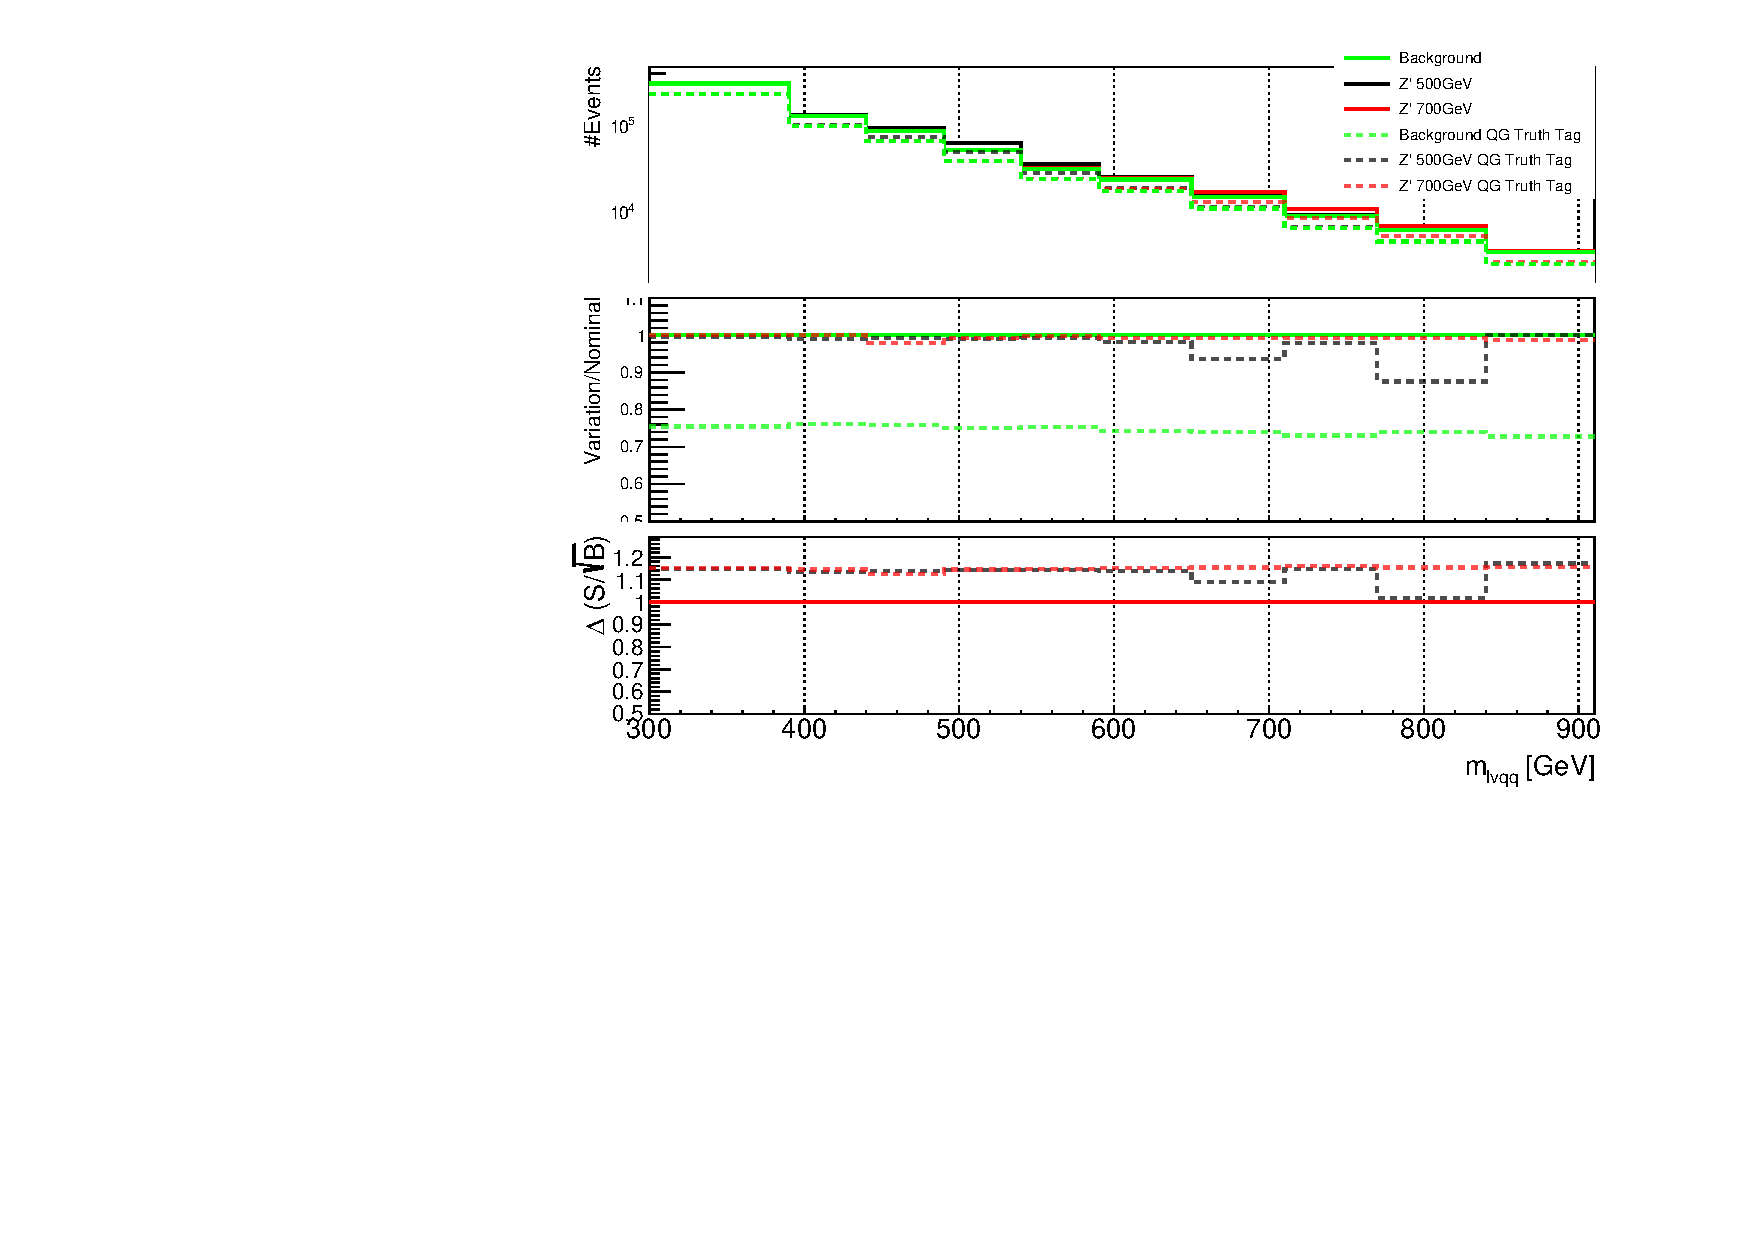
\includegraphics[width=\hsize]{figures/QGT/s_root_b_truthtag.pdf}
  \caption{The top panel shows the distribution of $m_{lvqq}$ with and without requiring jets to be true quarks. The middle panel shows the ratio of the signals and backgrounds with and without requiring jets to be true quarks. The bottom panel shows the change in $S/\sqrt{B}$ when requiring jets to be true quarks..}
  \label{fig:quark_gluon_roc_truth}
\end{figure}
\FloatBarrier



\begin{figure}[h!]
  \centering
  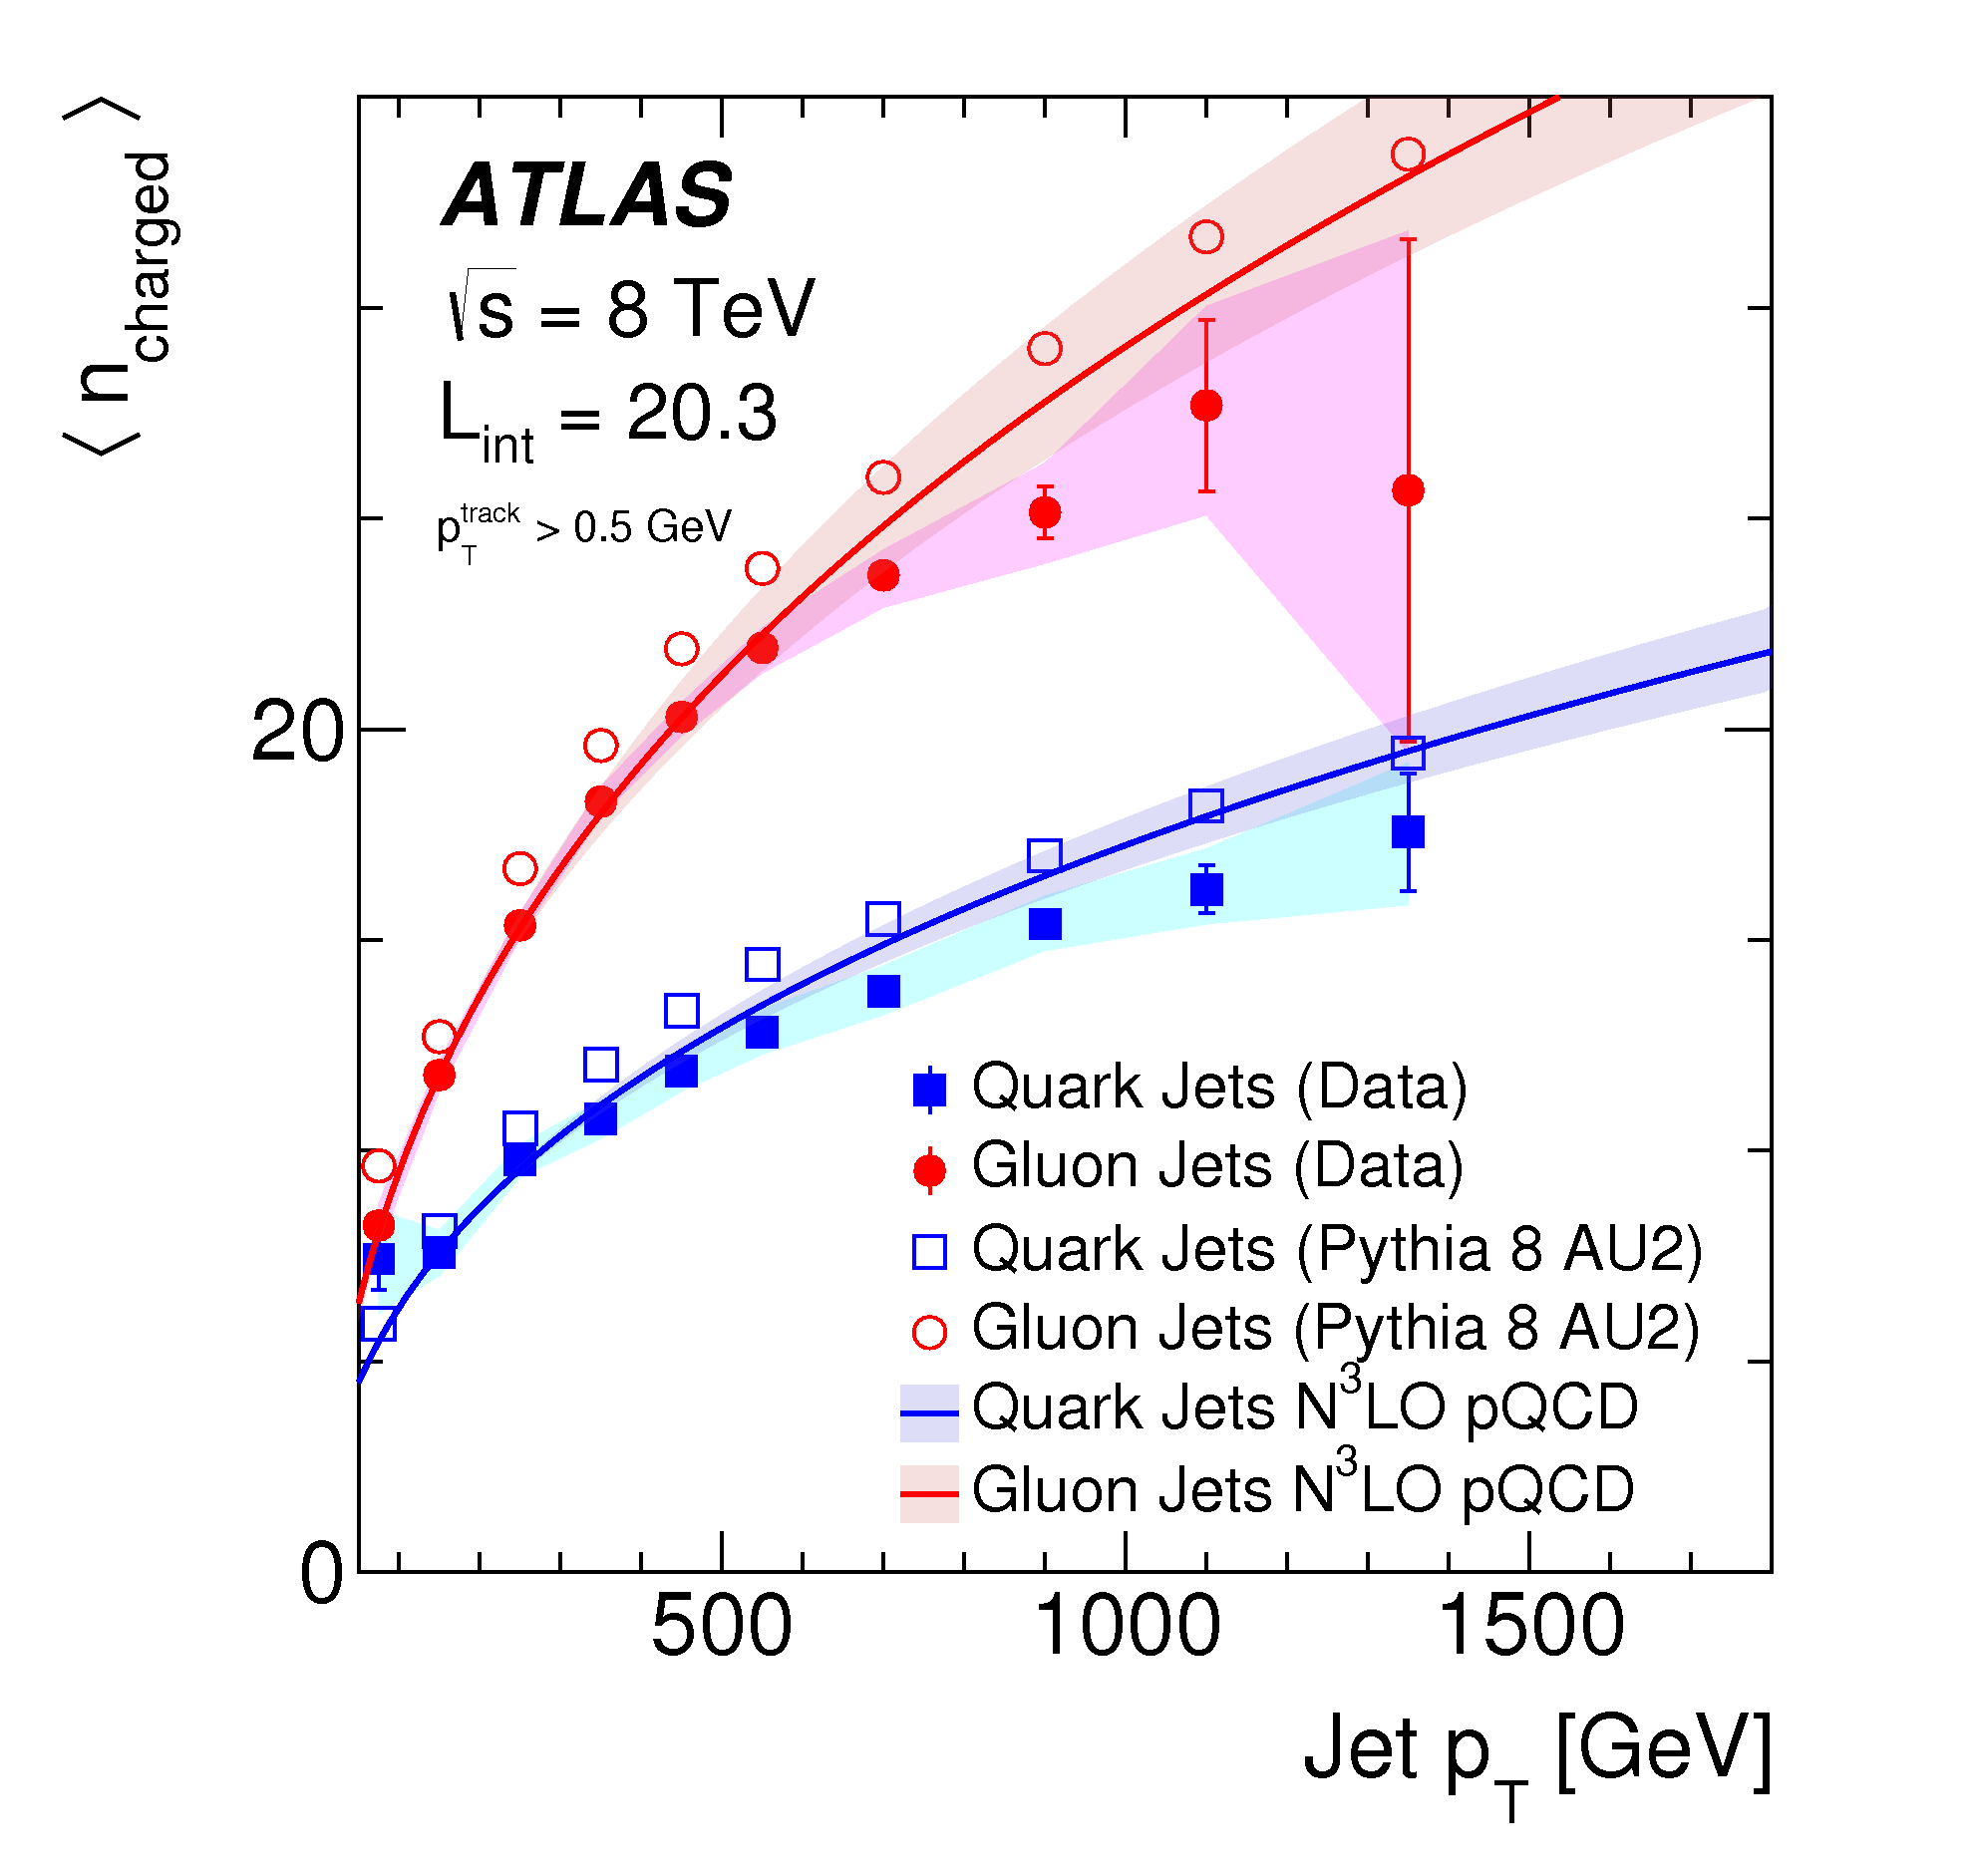
\includegraphics[width=\hsize]{figures/QGT/extracted_qg.png}
  \caption{Unfolded and extracted $n_{C}$ qg dstbs..}
  \label{fig:extracted_qg}
\end{figure}
\FloatBarrier



\begin{figure}[h!]
  \centering
  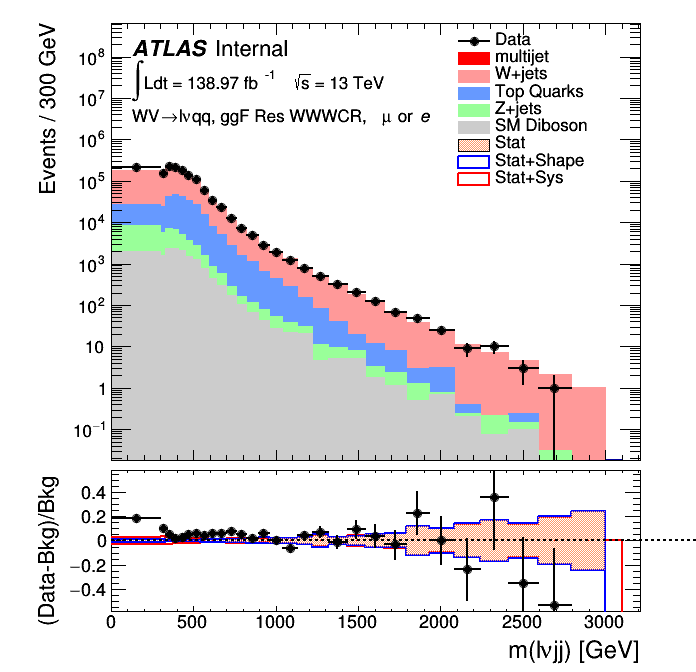
\includegraphics[width=0.45\hsize]{figures/QGT/C_0ptag2pjet_0ptv_ResolvedWWWCR_lvjj_m_Log.png}
 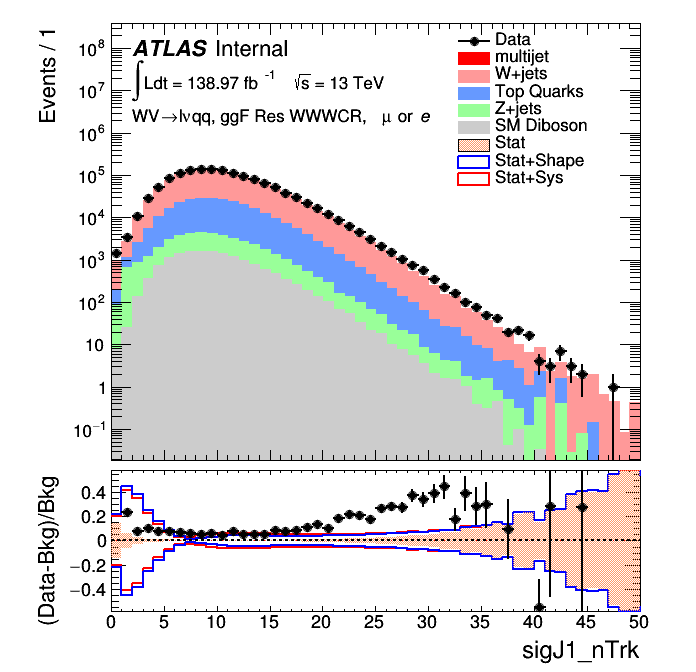
\includegraphics[width=0.45\hsize]{figures/QGT/C_0ptag2pjet_0ptv_ResolvedWWWCR_sigJ1_nTrk_Log.png}\\
   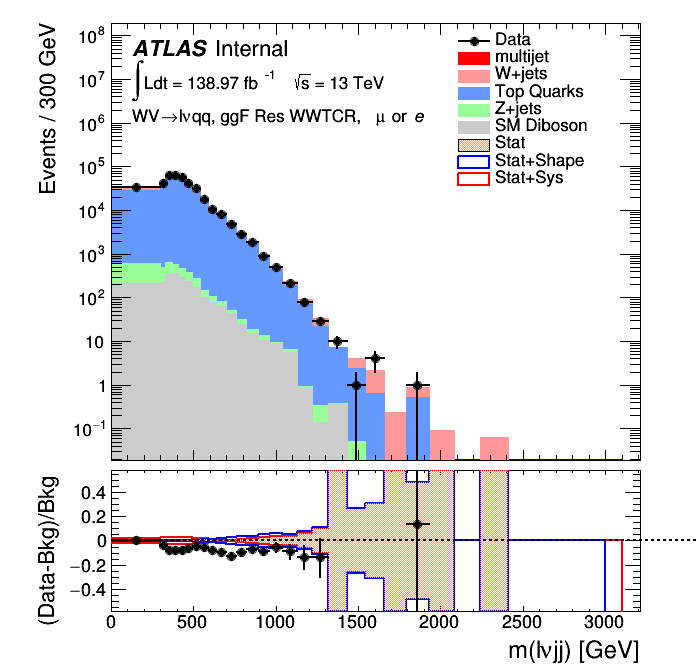
\includegraphics[width=0.45\hsize]{figures/QGT/C_0ptag2pjet_0ptv_ResolvedWWTCR_lvjj_m_Log.png}
 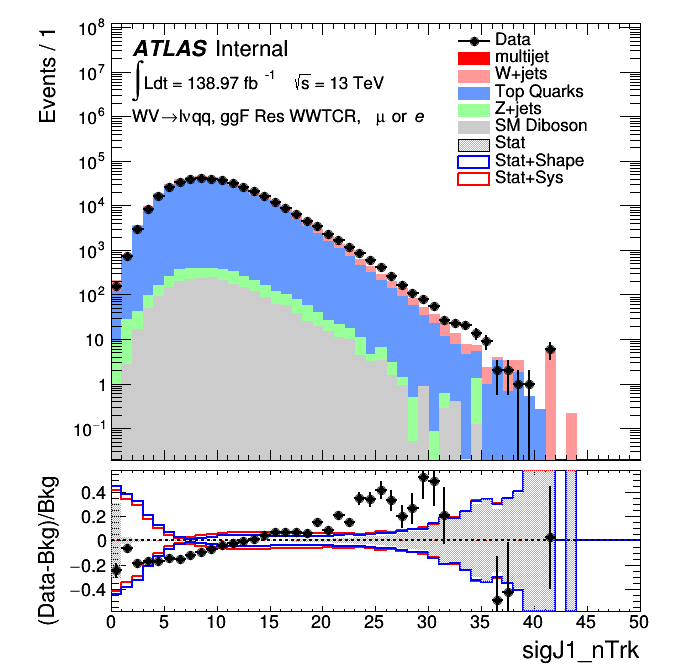
\includegraphics[width=0.45\hsize]{figures/QGT/C_0ptag2pjet_0ptv_ResolvedWWTCR_sigJ1_nTrk_Log.png}
 
  \caption{PDGID of the truth-level parton matched to the small-R jets passing the Resolved GGF WW Signal Region selections for the (a) Leading (b) Sub-Leading jets . These distributions are shown for 300, 500, and 700GeV Z' signals and the background.}
  \label{fig:qg_calib}
\end{figure}
\FloatBarrier



\begin{figure}[h!]
  \centering
  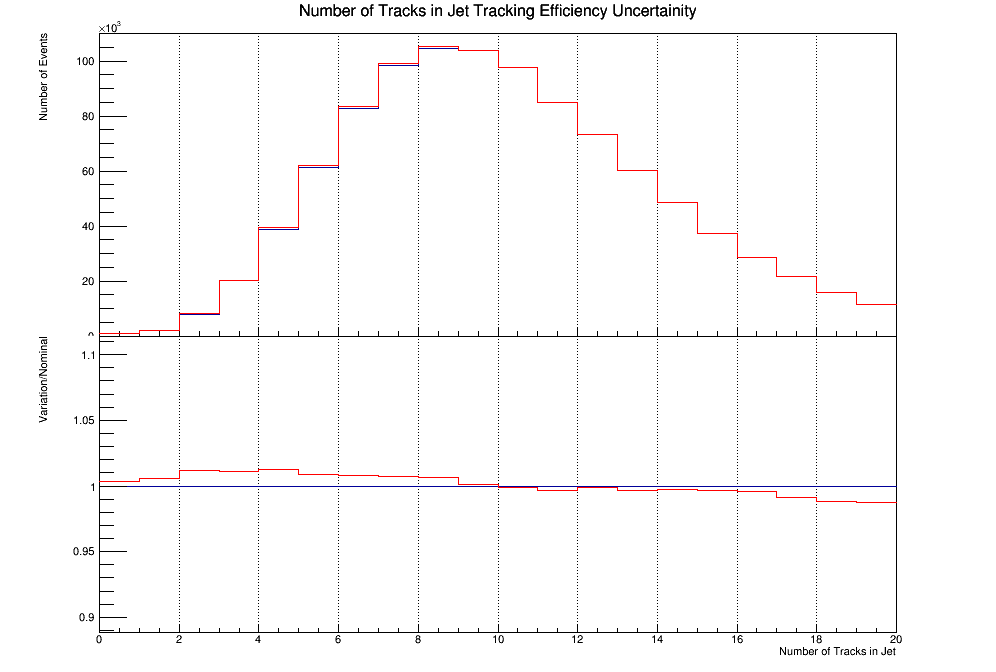
\includegraphics[width=0.45\hsize]{figures/QGT/sigWJ1_nTrkQG_trackeff.png}
 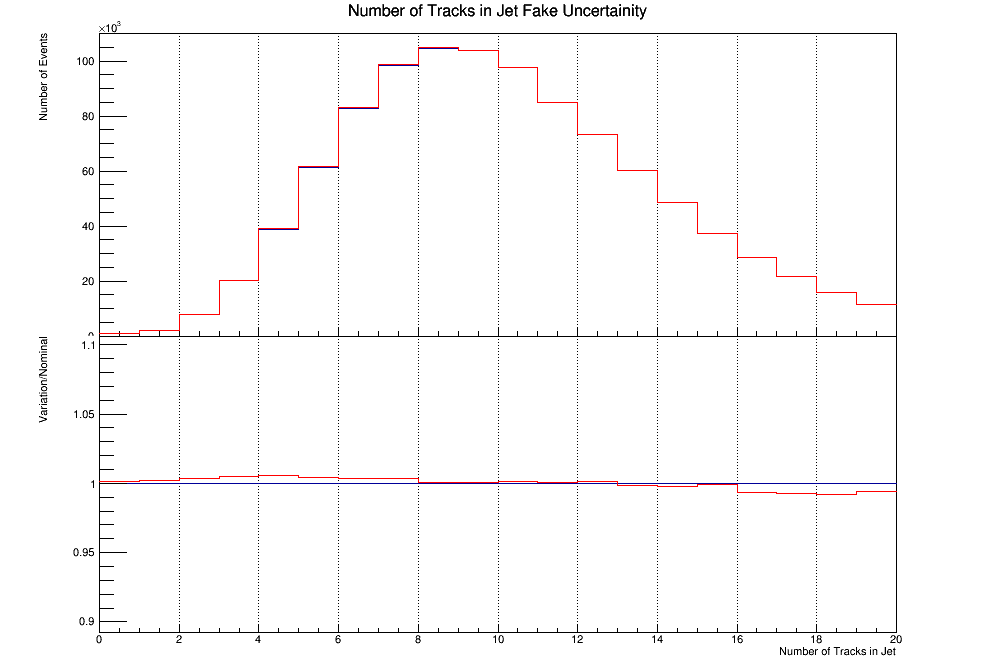
\includegraphics[width=0.45\hsize]{figures/QGT/sigWJ1_nTrkQG_fake.png}\\
   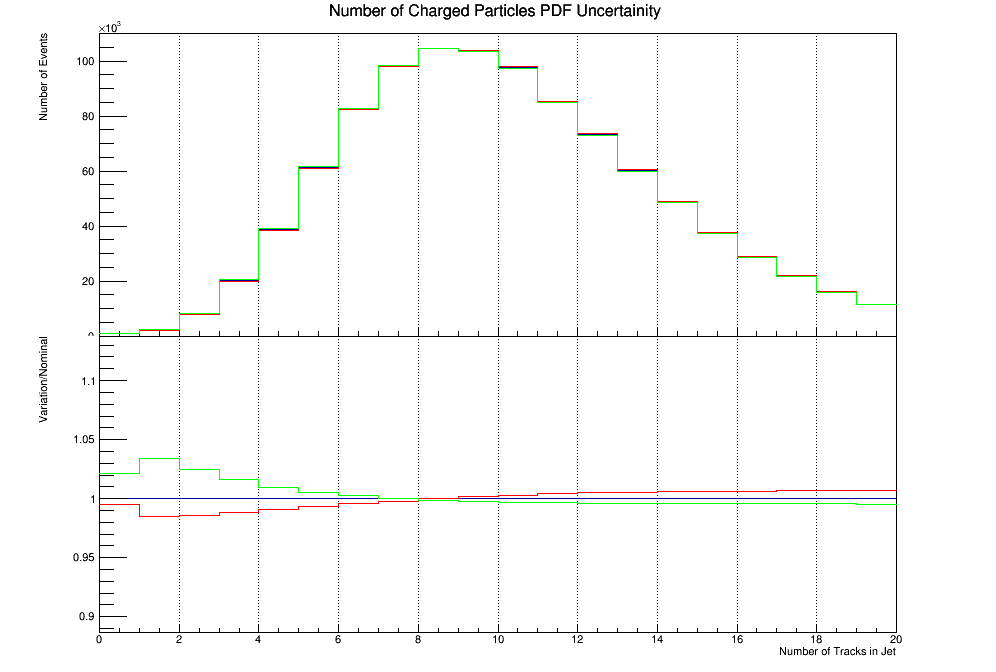
\includegraphics[width=0.45\hsize]{figures/QGT/sigWJ1_nTrkQG_pdf_up.png}
 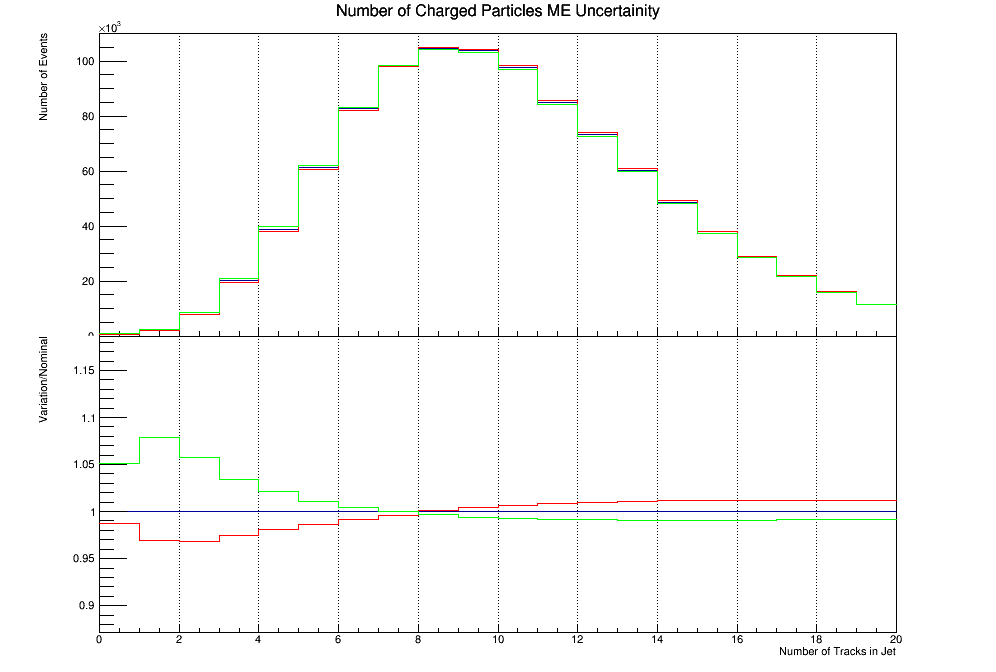
\includegraphics[width=0.45\hsize]{figures/QGT/sigWJ1_nTrkQG_me_up.png}\\
  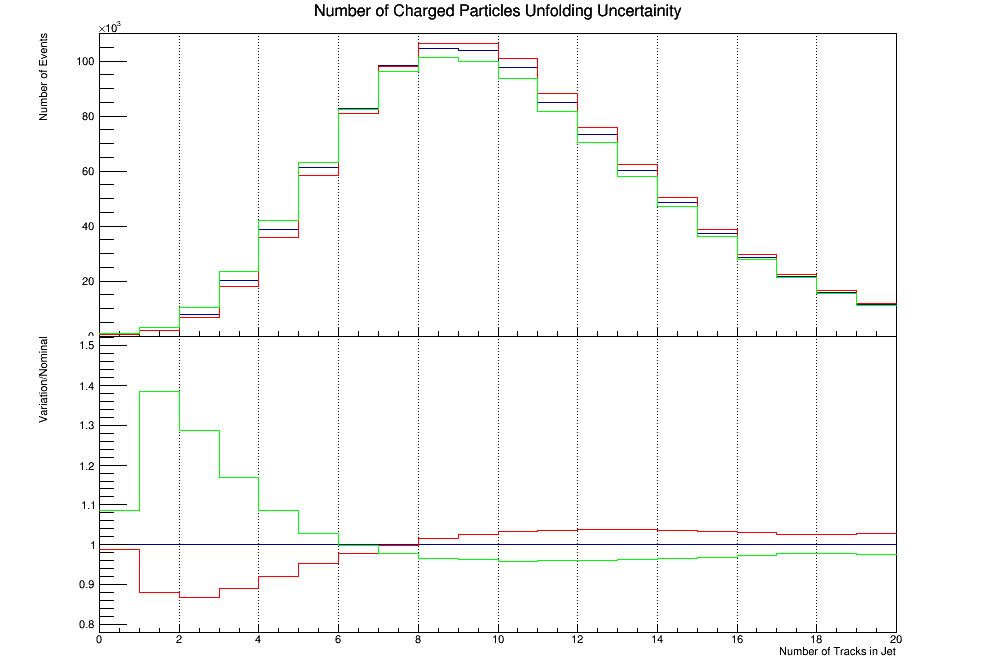
\includegraphics[width=0.45\hsize]{figures/QGT/sigWJ1_nTrkQG_exp_up.png}
 
  \caption{These figures show the impact of the uncertainities on the number of tracks in the leading jet in the sum of the background sample in the Resolved GGF WW SR (a) tracking efficiency (b) fake (c) PDF (d) ME (e) unfolding uncertainties.}
  \label{fig:qg_calib_ntrk_indiv}
\end{figure}
\FloatBarrier